\chapter{AN INTRODUCTION TO RECURRENT NUCLEOTIDE INTERACTIONS IN RNA}

RNA 3D motifs, folds and architectures are stabilized by a variety of
interactions between individual nucleotides (nts), primarily edge-to-edge base
pairing, face-to-face base-stacking and base-backbone interactions of various
kinds. Base-pairing is the most specific of these interactions, while
base-stacking provides much of the stabilization energy for RNA folding
\cite{Sponer2013}. In addition to the well-known Watson-Crick (WC) pairs,
structured RNA molecules contain many types of non-Watson-Crick (non-WC) base
pairs \cite{Leontis2001}. The non-WC pairs constitute a substantial fraction,
typically greater than one-third, of all base-pairs in a structured RNA
\cite{Stombaugh2009}. Familiarity with these and other recurrent
nucleotide-level interactions is fundamental for understanding RNA folding,
function, and evolution, because they are so widespread and crucial as building
blocks of RNA 3D motifs and complex RNA architectures. For example, analysis of
the recurrent geometries of non-WC pairs extends our understanding of the
patterns of sequence variation in homologous RNA molecules beyond the well-known
co-variation of Watson-Crick AU and CG base pairs \cite{Dutheil2010b,
Leontis2002f}.

To alert the reader to the importance of these interactions, we begin by
demonstrating their prevalence in the ``loops'' of the 2D representations of
structured RNA molecules, using \EC{} 16S rRNA as an example. Then we provide
detailed descriptions of the most important interactions. We introduce the
concept of base pair isostericity and show how to apply it to understand the
sequence variation of both WC and non-WC base pairs in homologous RNA molecules
and similar 3D motifs. We describe how to annotate 2D diagrams to capture the
most important interactions of RNA 3D motifs. Finally, we conclude by reviewing
on-line resources available through the Nucleic Acid Database (NDB) web portal
(\url{http://ndbserver.rutgers.edu/}) and related resources that provide access
to visualizations and comprehensive lists of interactions for all
atomic-resolution RNA structures in the Protein Data Bank (PDB), tools for
structure search, and compilations of 3D motifs organized by structural
similarity. 

\section{What about the Loops in RNA 2D diagrams?}

We begin with RNA secondary structure or ``2D'' diagrams, which are familiar to
most biochemists and molecular biologists. Strictly speaking, RNA 2D diagrams
are minimalist representations of the folding of the RNA chain on itself to form
the ``nested'' Watson-Crick (WC) base pairs. These representations generally omit
all other interactions, although they may display long-range pairs forming
pseudo-knots (PK), when these can be detected by comparative sequence analysis
(CSA). In cases with sufficient co-variation data, it has been possible to
extend secondary structures to include some non-WC pairs \cite{Gutell1994}. 

RNA 2D diagrams can be misleading in at least two ways: 
\begin{itemize}
  \item By implying that loops and linkers are single-stranded and that their
    nucleotides (nts) do not interact with the rest of the RNA in specific,
    phylogenetically conserved ways.

  \item By implying that RNA 3D structure is extended in 3D space with few or no
    interactions between different helical elements. 
\end{itemize}

Readers should note that 2D diagrams prepared before 3D structures were solved
continue to be widely used. Some of these 2D diagrams contain errors, especially
in the pairings of the most conserved bases that show little or no sequence
co-variation \cite{Petrov2013a}. Some WC pairs seen in the 3D structure are
absent in the 2D and some shown in the 2D are not found in the 3D. In addition,
some pairs shown as WC in the 2D actually assume non-WC geometries in 3D
structures. Discrepancies between 2D and 3D representations tend to occur either
adjacent to or within internal or multi-helix junction loops \cite{Petrov2013}.
There are at least five WC pairs in multi-helix junction loops of bacterial 16S
rRNA that are not shown in most 2D diagrams, and at least four of these could
not be detected by CSA. These are indicated with red lines in the 2D diagram of
\EC{} 16S rRNA shown in Figure~\ref{fig:ec-ssu-2d-3d}. This 2D representation is based on
annotations of nt interactions for NDB file RR0125 (PDB file 2AW7), as posted on
the NDB website (http://ndbserver.rutgers.edu/) and verified by visual analysis
of the 3D structure \cite{CoimbatoreNarayanan2014}. The corresponding helical elements in the 2D and 3D
representations of 16S rRNA are shown in Figure~\ref{fig:ec-ssu-2d-3d} highlighted with the same
colors. 

\begin{landscape}
  \begin{figure}
    \includegraphics[width=\linewidth]{chapter-1/figs/ec-ssu-2d-3d-converted}
    \caption{Structural representations of \EC{} 16S rRNA. 2D and 3D
      representations of 16S rRNA of \EC{} with helical elements colored
      identically. Lines connect WC paired nts. The 3D is PDB file 2AW7
      \cite{Schuwirth2005} while the 2D is modified from Petrov et al. 2013
      \cite{Petrov2013a}.}
    \label{fig:ec-ssu-2d-3d}
  \end{figure}
\end{landscape}

\subsection{Types of Loops }

The 2D structure partitions the nts of an RNA into disjoint sets constituting
helices, hairpin loops (HL), internal loops (IL), multi-helix junction loops
(MHJ), linkers, and 5’- or 3’-terminal sequences. Numbering the nts in a 2D
diagram consecutively from the 5’- to 3’-end makes it easy to find the helix,
loop or linker segment to which a given nt belongs. Hairpin loops occur at the
ends of helices and comprise continuous segments of RNA sequence linking the 3’
and 5’ strands at the ends of helices. Therefore they are also called terminal
loops, and many are found at or near the external surfaces of RNA molecules.
Certain types of HL, especially those with the consensus sequence, GNRA,
interact with other helical elements in the interior. Internal loops (IL) occur
between two helices and are composed of two strands. MHJ loops occur where three
or more helical elements meet. Linkers are single-stranded segments that connect
two domains or helical elements. 

To illustrate the importance of loop nts and their interactions in structured
RNA molecules, we analyzed the atomic-resolution structure of 16S rRNA from \EC,
as represented by a high quality, x-ray crystal structure, PDB file 2AW7
\cite{Schuwirth2005}. We examined the prevalence of loop nts, their
distributions and the number and types of interactions they form compared to
interactions of nts in WC-paired helices. 

\subsection{Distribution of nucleotides and their interactions}

Ribosome scientists partition the 16S rRNA 2D structure into about 50 helical
elements, connected to each other by MHJ or by single-stranded linkers. Each
helical element comprises one or more helices, connected to each other by IL. Of
these, 32 helical elements terminate on one end in HL as shown in
Figure~\ref{fig:ec-ssu-2d-3d} \cite{Petrov2013a,Yusupov2001}. A further 17 serve to
connect two MHJ (for example, helices 4 and 5 in 16S rRNA) or a MHJ and
single-stranded linkers (for example, helix 28). An additional helical element
of 16S, helix 2, constitutes a pseudo-knot and is not considered part of most 2D
representations of 16S. More than half of the helical elements are interrupted
by one or more internal loops (IL). H44, the longest helical element in 16S and
a prominent part of the 30S interface with the 50S subunit, for example,
contains nine IL. The large number of IL in \EC{} 16S (63, see
Table~\ref{tab:ec-element-count}) accounts for the larger number of helices
(\textasciitilde 111), defined as uninterrupted WC-paired duplexes, compared to helical
elements (\textasciitilde 50), and the prevalence of very short ``helices,'' consisting of
less than three base pairs. 

\begin{table}[ht]
  \begin{tabular}{llrr}
    \toprule
    16S rRNA Elements     & Number of Elements & Number of Nucleotides  & Percentage of Total Nucleotides \\
    \midrule
    Hairpin loops         & 32                 & 172                    & 11.24 \\
    Internal loops        & 63                 & 256                    & 16.73 \\
    Multi-helix junctions & 17                 & 197                    & 12.88 \\
    Linker segments       & 8                  & 39                     & 2.55 \\
    Total ‘loop’ nts      & 11                 & 664                    & 43.40 \\
    Helices               & 111                & 866                    & 56.60 \\
    Total nts             &                    & 1530                   & 100.00 \\
    \bottomrule
  \end{tabular}
  \caption{Summary of the 2D Structure of \EC{} 16S rRNA,
    updated with Base-Pairing Annotations from the NDB Entry for 2AW7 and Manual
  Analysis of the 3D Structure.}
  \label{tab:ec-element-count}
\end{table}

Table~\ref{tab:ec-element-count} presents the distribution of nts based on the
corrected 2D structure of \EC{} 16S rRNA (Figure~\ref{fig:ec-ssu-2d-3d}) and the
analysis of annotations of NDB file RR0125 (PDB file 2AW7). This 3D structure
has 1530 nts, 12 nts less than the accepted total for \EC{} 16S (1542), because
some of the nts on the 5'- and 3'-ends are not resolved in this structure, which
also lacks tRNAs and mRNA. 

The most significant result in Table~\ref{tab:ec-element-count} is that fully
43.4\% of the nts of \EC{} 16S belong to the loop or linker regions. The
remaining 56.6\% of nts form the nested AU, GC, and GU Watson-Crick (WC) base
pairs that constitute the helices defining the 2D structure. The structure
contains an additional twelve WC base pairs forming long-range tertiary (3°)
interactions, in addition to the five pairs mentioned above that are integral
parts of multi-helix junction loops. The 34 nts forming these 17 tertiary WC
pairs are assigned to their respective loop or linker segments rather than to
the helices of the 2D structure. Regarding the distribution of nts in different
kinds of loops, comparable numbers of nts constitute the HL (11.2\%) and MHJ
loops (12.9\%), while the IL have somewhat more nts (16.7\%). The remaining nts
belong to linker regions (2.6\%). In the category of single-stranded linkers, we
include the 5' and 3' ends of the molecule. In summary, more than 40\% of the
nts of 16S rRNA belong to loops or linkers. Next we examine the size
distributions of helices and loops. 

\subsubsection{Size distributions of helices and loops}

Figure~\ref{fig:ec-helix-lengths} shows the distribution, in base pairs (BP), of
the lengths of 16S helices. Most helices in 16S are surprisingly short,
comprising four or fewer base pairs. This is not atypical of structured RNA
molecules. The longest continuous helices in \EC{} 16S, uninterrupted by
internal loops or single-base bulges, are only 12 base pairs long and a
significant number of ``helices'' consist of only one or two WC base pairs.
Reasons for including these very short helices in the 2D structure are discussed
below. 

\begin{figure}
  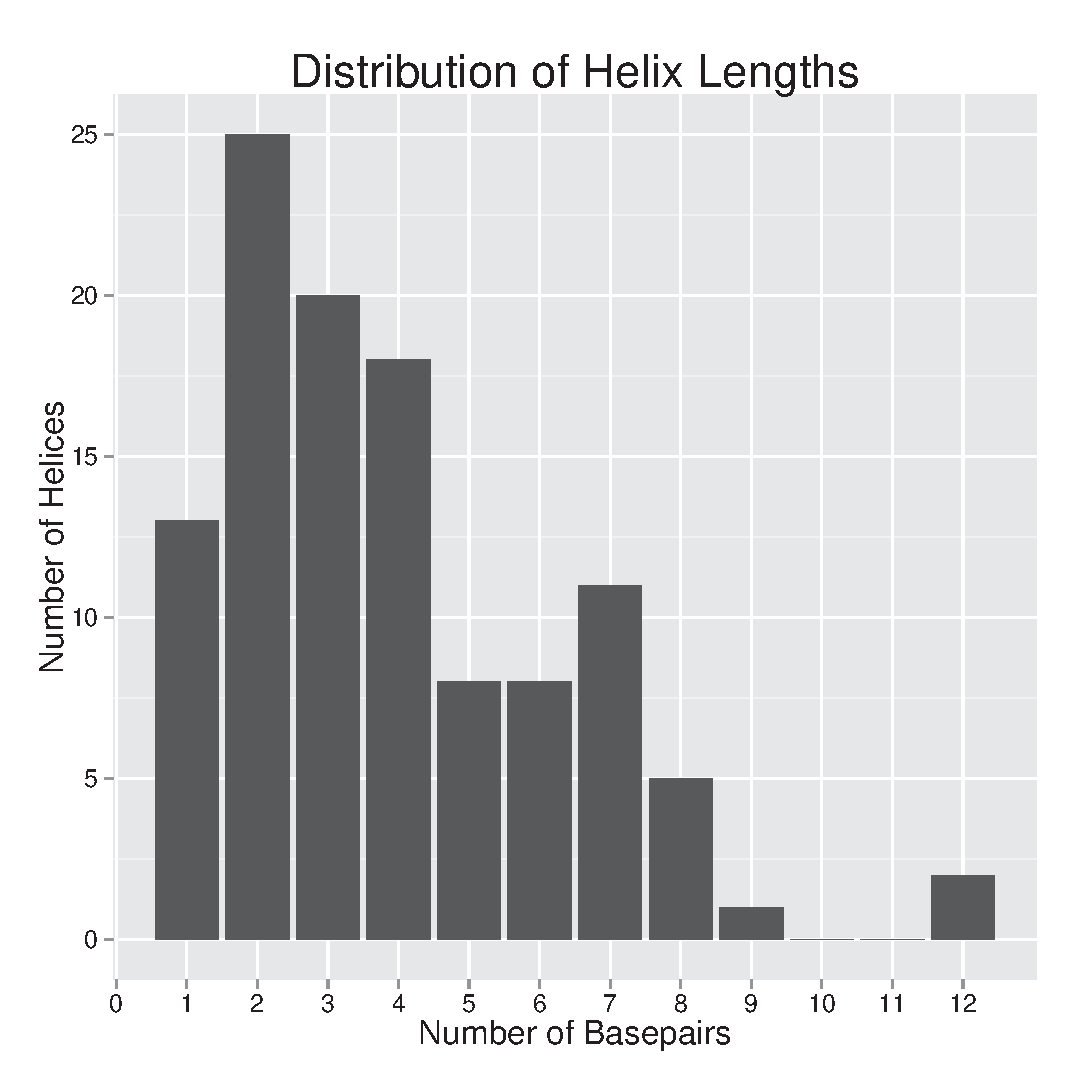
\includegraphics[width=0.5\linewidth]{chapter-1/figs/helix-lengths.eps}
  \caption{Distribution of Helix Lengths in 16S rRNA. Histogram of helix lengths
    (in base pairs) from the 2D representation of 16S rRNA in
  Figure~\ref{fig:ec-ssu-2d-3d}, using definitions of helices explained in the
text.}
  \label{fig:ec-helix-lengths}
\end{figure}

Figures~\ref{fig:ec-hl-sizes} and \ref{fig:ec-il-sizes} show the size
distributions of HL and IL in 16S rRNA. Many HL in 16S rRNA comprise 4 nts and
almost all of these are recurrent GNRA or UNCG type loops \cite{Woese1990a}. The
smallest HL is just 2 nts. In this loop, the closing base pair is Watson-Crick
and is not counted as part of the HL. Recurrent GNRA and UNCG HL are closed by
non-WC paired nts, which are counted as parts of these loops; therefore, GNRA
and UNCG HL also have just two unpaired nts. 

\begin{figure}
  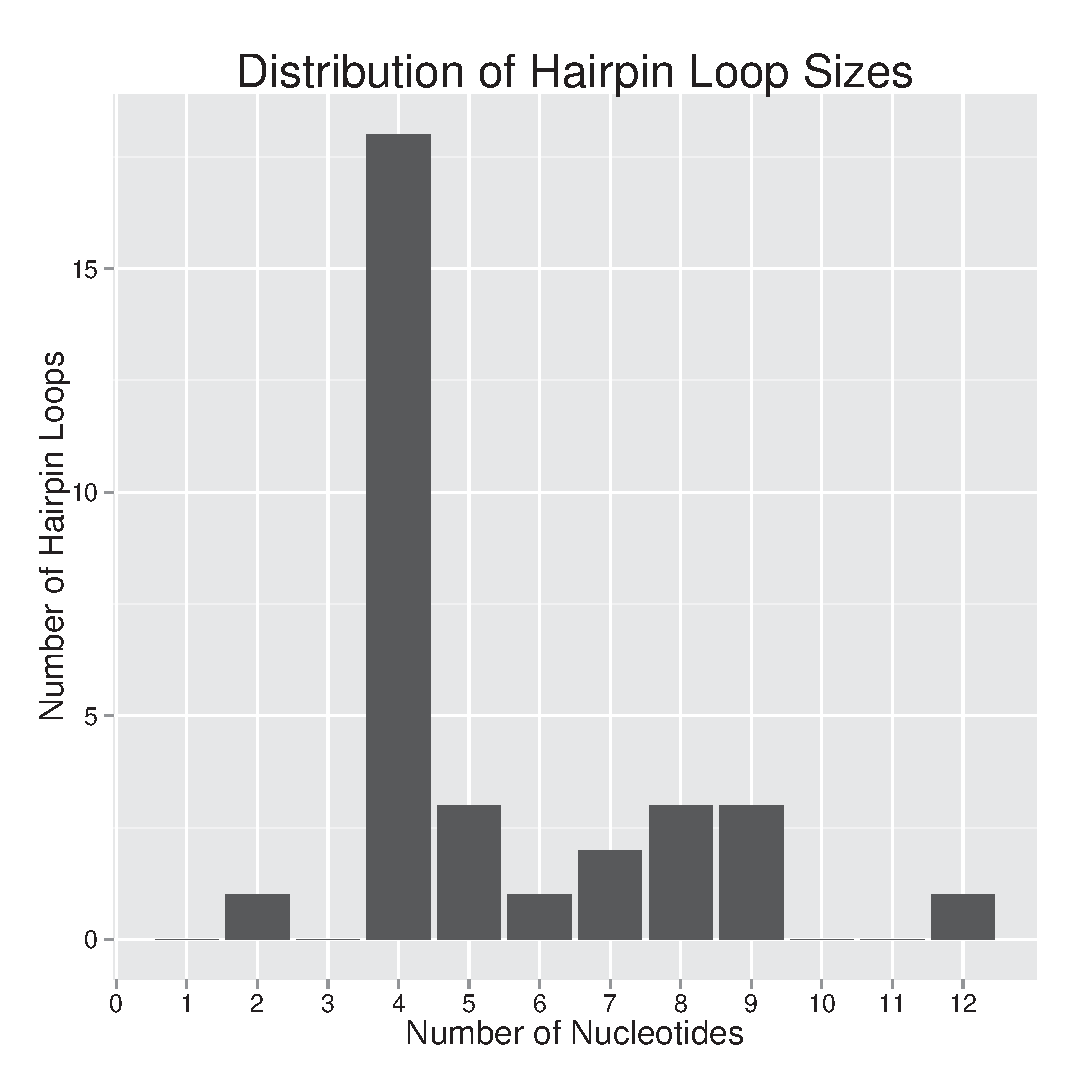
\includegraphics[width=0.5\linewidth]{chapter-1/figs/hl-sizes}
  \caption{Distribution of Hairpin Loop Sizes in 16S rRNA. Histogram of HL sizes
    (in nts) from the 2D representation of 16S rRNA in
  Figure~\ref{fig:ec-ssu-2d-3d}.}
  \label{fig:ec-hl-sizes}
\end{figure}

\begin{figure}
  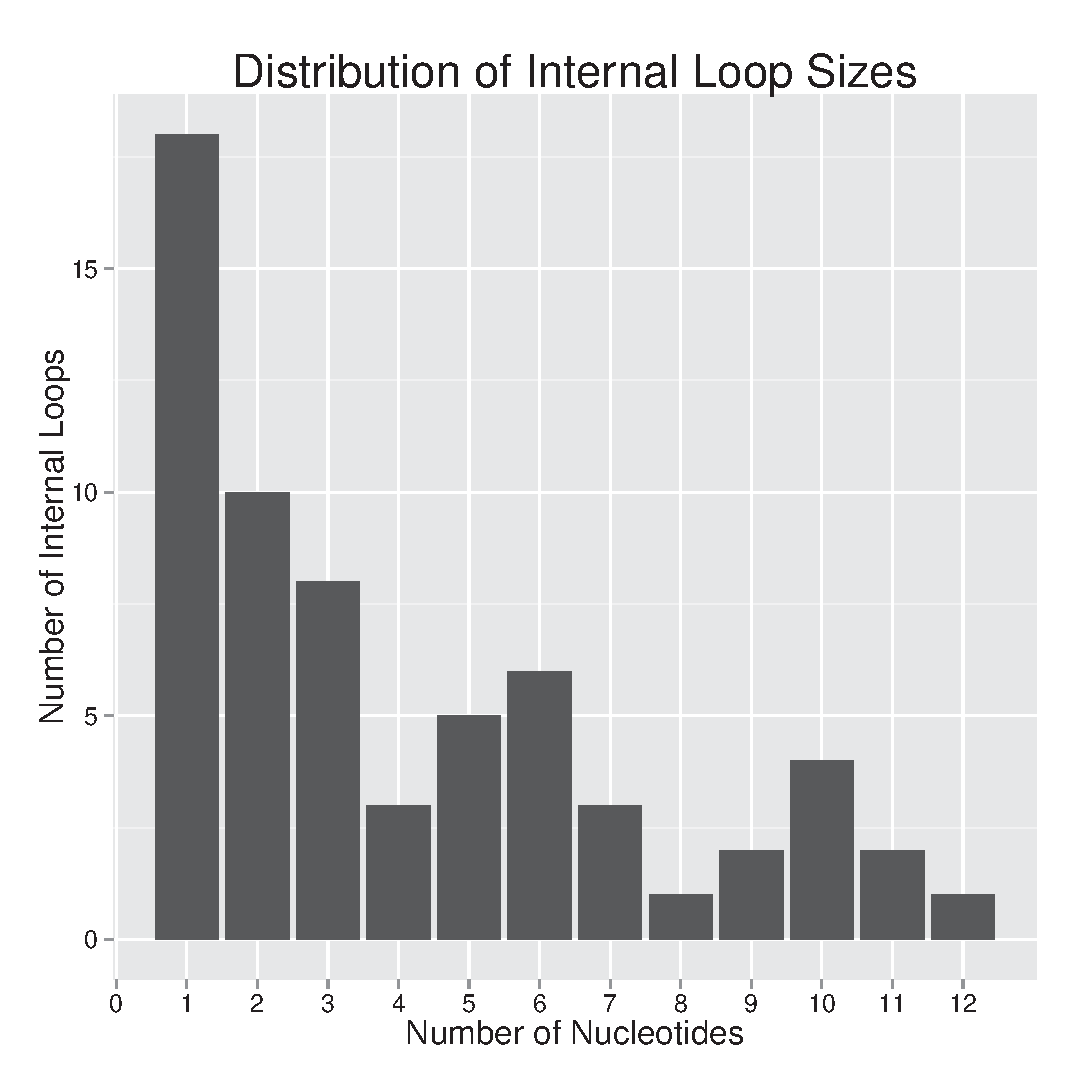
\includegraphics[width=0.5\linewidth]{chapter-1/figs/il-sizes}
  \caption{Distribution of Internal Loop Sizes in 16S rRNA. Histogram of IL
  sizes (in nts) from the 2D representation of 16S rRNA in
  Figure~\ref{fig:ec-ssu-2d-3d}.}
  \label{fig:ec-il-sizes}
\end{figure}

The smallest IL consists of just one ``bulged'' nt, flanked on each side by
Watson-Crick base pairs. There are several of these in 16S rRNA and almost all
of them are very conserved \cite{Gutell1994}. The 2D diagram implies that each
of these is ``bulged'' out. While the 3D structure shows that some are indeed
bulged out, others form specific interactions with the adjacent WC base pairs or
intercalate between them. Thus, even the simplest IL, drawn identically in 2D
diagrams, give rise to different, geometrically distinct 3D motifs. IL having
two nts can be symmetric (1x1), with one nt in each strand, or asymmetric (2x0)
with both loop nts in one strand. Again, each of these 2D motifs gives rise to
different, structurally distinct 3D motifs. To classify loop motifs in
functionally meaningful ways, the types of interactions that the loop nts form
among themselves must be considered. Using this approach, all HL and IL loops
extracted from unique NDB structures have been classified by structural
similarity and organized into an RNA Motif Atlas \cite{Petrov2013}. The RNA
Motif Atlas can be accessed through the redesigned NDB website
\cite{CoimbatoreNarayanan2014}, and will be discussed in the last section of
this review.

\subsubsection{Interactions of loop nucleotides}

Using 16S rRNA as an example, it was shown in the previous sections that
substantial fractions of nts in structured RNAs belong to ``loops'' and these
vary in size and structure. Next, we examine the roles that loop nts play in RNA
3D structures. Figures~\ref{fig:ec-bp-loop-v-helix} and
\ref{fig:ec-inter-loop-v-helix} provide histograms to compare the number of
interactions involving loop vs. helix nucleotides.
Figure~\ref{fig:ec-bp-loop-v-helix} shows base pair interactions and
Figure~\ref{fig:ec-inter-loop-v-helix} shows all annotated inter-nucleotide
interactions, including base-pairing, base-stacking and base-phosphate
interactions. Each type of interaction will be described in more detail below.
Two important points emerge from Figure~\ref{fig:ec-bp-loop-v-helix}: (1) More
than 50\% of ``loop'' nucleotides form one or more base pairs. (2) A significant
fraction (9\%) of helix nts makes one or two additional base pairs, in addition
to the defining Watson-Crick pair each forms. The additional base pairs involve
base edges other than the Watson-Crick edge and are, by definition, non-WC
pairs. In no case do bases make more than three base pairs, for reasons
explained below.

\begin{figure}
  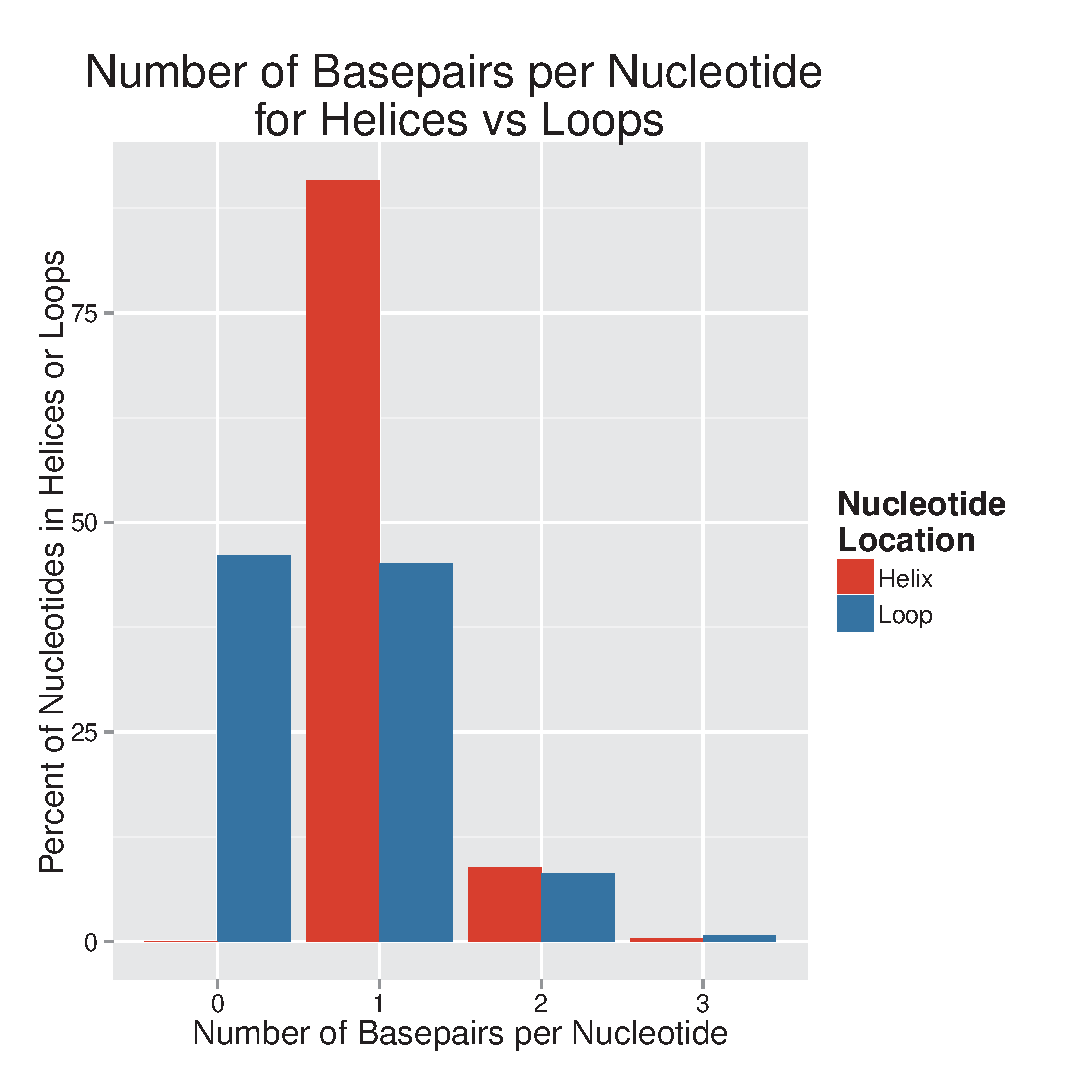
\includegraphics[width=0.5\linewidth]{chapter-1/figs/bp-loop-v-helix}
  \caption{Comparison of Base pairs formed by Nucleotides in Loops vs. Helices.
    Histogram comparing number of base pairs (non-WC as well as WC) formed by
  nucleotides in loops (blue) vs. helices (red).}
  \label{fig:ec-bp-loop-v-helix}
\end{figure}

\begin{figure}
  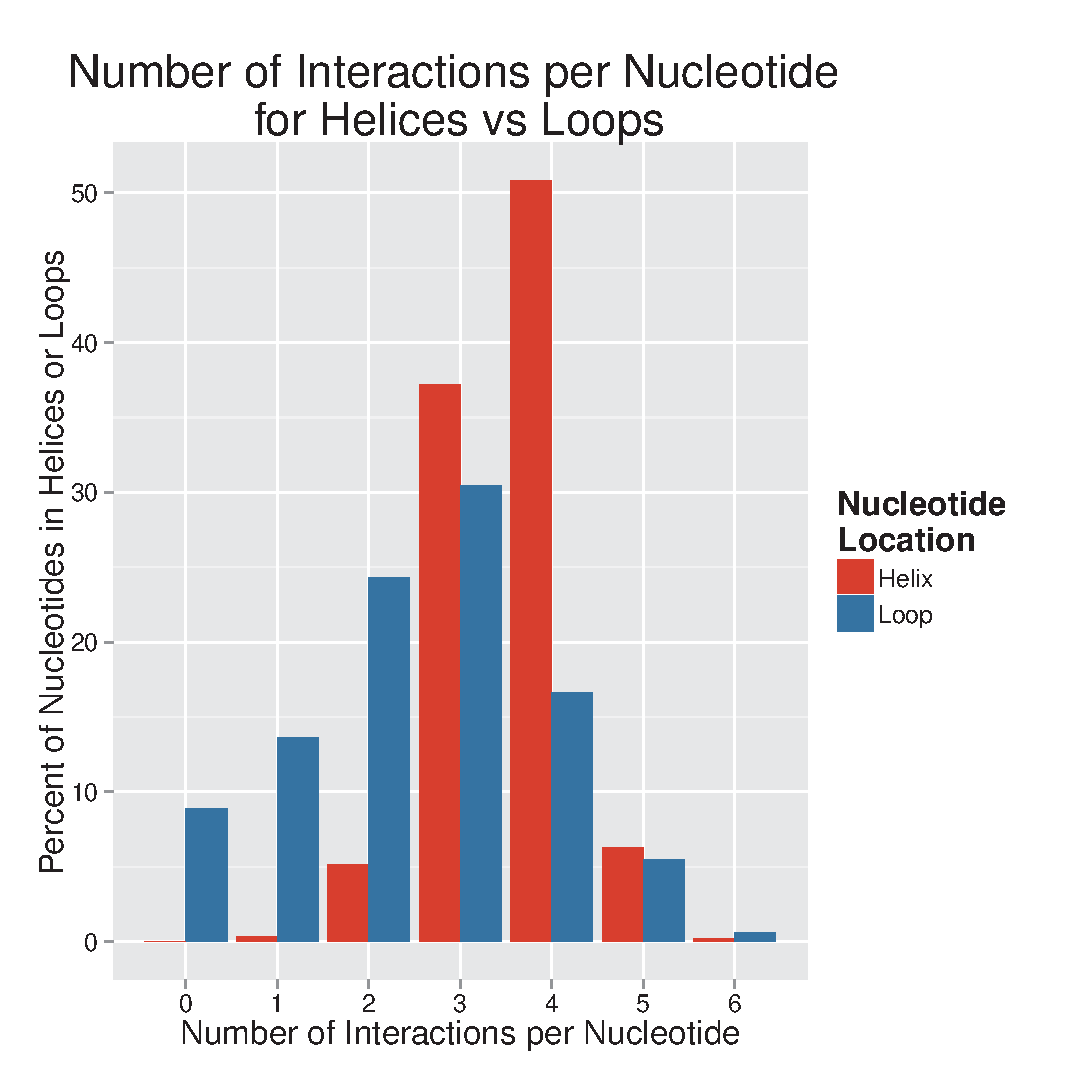
\includegraphics[width=0.5\linewidth]{chapter-1/figs/inter-loop-v-helix}
  \caption{Comparison of Interactions formed by Nucleotides in Loops vs.
  Helices. Histogram comparing number of annotated interactions (base-pairing,
base-stacking, and base-phosphate) formed by nucleotides in loops (blue) vs.
helices (red).}
  \label{fig:ec-inter-loop-v-helix}
\end{figure}

Figure~\ref{fig:ec-inter-loop-v-helix} shows that when we include stacking and
base-phosphate interactions, most nts in the 16S structure, whether they are
found in loops or helices, form two or more interactions. As expected, most
helix nts form 3 or 4 interactions, corresponding to one base pair and 2 or 3
stacking interactions per nt. Even nts on the ends of helices stack on at least
one other base. Thus, almost all helical nts have at least two interactions, one
pairing and one stacking. With regard to loop nucleotides,
Figure~\ref{fig:ec-inter-loop-v-helix} shows that almost 80\% form two or more
interactions with other nts in 16S rRNA | evidence that most loops form specific
structures. On average, nucleotides in loops form
2.5 interactions per nt compared to 3.6 for those in helices. The stacking data
(not shown) shows that 85\% of loop nts form one or more stacking
interactions, with >60\% forming two or more; on average, loop nts form 1.7
stacking interactions per nucleotide, compared to 2.5 for helix nts. 

Less than 15\% of loop nts form only 1 interaction and, surprisingly, only \textasciitilde 58
loop bases in 2AW7, or less than 4\% of all nts in this 16S rRNA structure, form
no classified pairing, stacking or base-backbone interactions and are candidates
for bases that completely “bulge out” of the structure, as implied by 2D
diagrams for all loop nts. Detailed analysis of 3D structures of ribosomes in
different states shows that most of these 58 bases do in fact form some kind of
interaction by stacking or H-bonding to tRNA, mRNA or 23S rRNA, by binding to
ribosomal proteins, or by forming as yet unannotated or unclassified base-ribose
or perpendicular base-base interactions with other nts (Roy et al., unpublished
observations). Classification of base-ribose and perpendicular interactions is
an active area of research (Zirbel, private communication); once classes of
interactions are agreed upon, these interactions will also be annotated in NDB. 

Regarding base-phosphate (BPh) interactions, which are the most sequence
specific base-backbone interactions, less than 4\% of helical nucleotides (34 of
866) provide the base in such interactions, whereas 18.4\% of loop bases do so
(122 of 664). In addition, 18\% of loop nts provide the phosphate groups for BPh
interactions but only 4\% of helix nts do so. This shows that loop nts also play
a prominent role in mediating BPh interactions, which contribute substantially
to stabilizing folded RNA structures \cite{Zirbel2009, Sponer2010}. 

Taken as a whole, these data show that nts in loops and linkers form significant
numbers of interactions of all types and therefore loop regions are generally
well structured and contribute significantly to RNA 3D structure. Next we
analyze these interactions in more detail to identify the locations of
interacting nucleotides. 

\subsection{Local vs. long-range interactions in loops and helices}

To better understand the roles of loop and linker nts in RNA 3D structure, we
next address these questions: How many structure-stabilizing interactions occur
between loop nts, how many between helical nts, and how many between loop and
helical nts? How many of these interactions contribute to local structure and
how many to the overall 3D architecture? To answer these questions it is useful
to classify interactions according to whether they are local or long-range.
Long-range interactions are of particular interest because they contribute to
the overall folding of structured RNA molecules. Before presenting the data, we
discuss how local and long-range interactions can be distinguished by automated
means to facilitate structural analysis (Zirbel, private communication). 

\subsubsection{Defining long-range (LR) interactions}

Local interactions are those between nts belonging to the same helix or loop, or
between adjacent elements of the 2D structure, while LR interactions are those
between nts distant in the 2D. The farther apart two nts are in the 2D
structure, the more WC base pairs they ``cross over'' when they interact. By
definition, all of the WC base pairs that define the 2D structure are ``nested''
with respect to each of the others.  Two WC pairs (i,k) and (m,n) are nested
when either i \textgreater m \textgreater n \textgreater k (as shown in
Figure~\ref{fig:nesting}A) or m \textgreater i \textgreater k \textgreater n,
where i, k, m and n are the nt numbers in the linear RNA sequence (given in the
5’ to 3’ direction) and i \textgreater k, m \textgreater n. In other words,
nested interactions do not cross over each other in the 2D structure. On the
other hand, if two interactions (i,k) and (m,n) are such that i \textgreater m
\textgreater k \textgreater n, as shown in Figure~\ref{fig:nesting}B, or
alternatively, m \textgreater i \textgreater n \textgreater k, then they
``cross.'' Once a comprehensive set of nested WC pairs is identified and
assigned to the 2D structure, one can measure how ``local'' or ``LR'' any other
interaction is, by counting the number of nested WC pairs it crosses over. This
measure is called the “crossing number,” and the larger it is, the more distant
the interacting nts are in the 2D structure.  By definition, all WC pairs that
belong to the 2D structure have crossing number equal to zero. An example of an
interaction (x,y) that crosses two nested Watson-Crick pairs, (i,j) and (m,n),
is shown in Figure~\ref{fig:nesting}C. The pair (x,y) has crossing number equal
to two. Whether interactions are labeled local or LR depends on the choice of
cutoff for the crossing number. Certainly, the cutoff should be $\ge 1$, so that
interactions with crossing number zero are labeled ``local.'' The smaller the
cutoff, the more interactions will be defined as LR, but if the cutoff is set
too low, interactions between nts that are very close to each other in the 2D
structure and best considered local, will be labeled LR. If the cutoff is set
too high, interactions best classified as LR will be labeled local. We find that
a cutoff equal to four provides a good compromise, so we label all interactions
with crossing number $\ge 4$ ``LR'' (Zirbel, private communication). 

\begin{figure}
  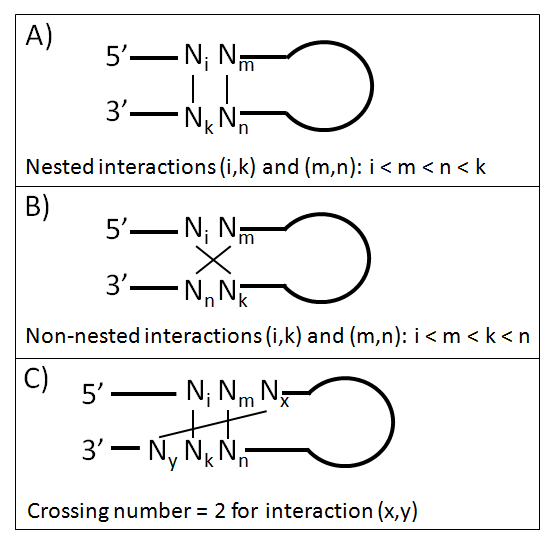
\includegraphics[width=0.5\linewidth]{chapter-1/figs/nested}
  \caption{Definition of Crossing Number for Long-range Interactions. Base pairs
    (i,k) and (m,n) are nested in (A) but non-nested in (B). Interaction (x,y)
    in (C) crosses over two nested base pairs, (i,k) and (m,n) and has crossing
  number equal to 2.}
  \label{fig:nesting}
\end{figure}

\subsubsection{Local vs. long-range (LR) interactions in 16S rRNA}

Using crossing number $\ge 4$, we find 163 LR interactions in 16S rRNA. The
relevant data for \EC{} 16S rRNA are presented in Table 2. Not surprisingly,
most nt interactions are local (2323 local vs. 163 long-range) and most of these
are between two nts in the same or adjacent helices (1323 out of 2323 or 57\%);
however, almost 24\% of local interactions are between nts in the same or nearby
loops (552/2323) and 19\% (448/2323) involve nts in adjacent loops and helices.
Most such local loop-helix interactions are base stacking (386 of 448 or 86\%),
indicating that loop nts frequently stack with the WC pairs of adjacent helices.
Many of these helices appear in the 2D to be very short, comprising only one or
two base pairs (see Figures \ref{fig:ec-ssu-2d-3d} and
\ref{fig:ec-helix-lengths}). Thus, for the most part, these very short helices
are not isolated but are stabilized by stacking on bases in the adjacent HL, IL
or MHJ loops, many of which form non-WC base pairs. In fact, 16S rRNA contains
15 local AG cis Watson-Crick (cWW) base pairs, most of which occur at the
interfaces between loops and helices. Readers should note that cWW pairs
composed of non-canonical base combinations (i.e. other than AU or GC) are
considered non-WC pairs. These and other non-WC pairs can be considered to
form extensions of the secondary structure \cite{Gutell1990}. Local stacking
interactions also play major roles in loops; they account for 336/552 or 61\%
of interactions within loops. In fact, 336/1600 (22\%) of all local stacking
interactions occur in loops. 

As concerns local pairing and base-phosphate interactions in loops, most of
these occur between nts in the same or adjacent loops and far fewer with nts in
helices (135 local loop-loop vs. 38 local loop-helix base-pairing interactions
and 81 local loop-loop vs. 24 local loop-helix BPh interactions). 

While there are far fewer LR than local interactions within 16S rRNA, the LR
contacts are crucial for defining and stabilizing the 3D architecture. The
absolute numbers depend, of course, on the value of the crossing number cutoff
used, as discussed above. In generating the data reported here, we used cutoff =
4. With this cutoff, most LR interactions occur between nts distant in the 2D
structure, i.e. nts belonging to different helical elements and even
different structural domains. While 76\% of local interactions involve helix
nts (1771 of 2323 interactions), 93\% of long-range interactions involve loop
nts (157 of 168) of which 52\% (87 of 168) are between two loop nts.  Only
11/168 or 6.5\% of long-range interactions are between two helix nts and all
of these are BPh or helix packing  (``P-'') interactions \cite{Mokdad2006b}.
The latter involve highly conserved GU pairs that interlock on their sugar
edges with AU or GC WC pairs and occur exclusively between helices, forming
crucial highly conserved inter-helical tertiary contacts in structured RNAs
\cite{Gagnon2006, Gagnon2002}. 

Table 2 shows that LR loop-loop interactions include comparable numbers of
pairing, stacking and BPh interactions, while LR loop-helix interactions are
dominated by non-WC base pairing. Most of these involve the sugar edges of the
helix nts (see below). 

In base-phosphate (BPh) interactions, one nt contributes the base and the other
the phosphate group. The base-phosphate interactions are separated in Table 2
according to whether the helix or loop nt contributes the base to the
interaction. The row in Table 2 labeled ``Helix-Loop'' includes interactions in
which the helical nts contribute the base and vice versa for the row labeled
``Loop-Helix.'' These data show that the loop nt usually provides the base in LR
loop-helix BPh interactions, whereas this is reversed in local interactions.
There are comparable numbers of LR base-pairing and LR BPh interactions between
loops and helices as between two loop nts, but far more LR stacking interactions
between two loop nts than between loop and helix nts interactions (34 vs. 6). 

\subsubsection{Base-stacking interactions of loop nts}

What kinds of stacking interactions are observed in loops? As in helices, there
is stacking between consecutive bases in the same strand, but in loops there are
additional types of stacking. In many loops, there is extensive “cross-strand”
stacking between bases forming consecutive non-WC base pairs but located in
opposite strands. Cross-strand stacking is a characteristic feature of many RNA
3D motifs, including recurrent sarcin-ricin motifs \cite{Szewczak1993a}.
Extensive stacking is also observed between helical elements that meet at MHJ.
As helices at MHJ can stack in different ways, the pattern of inter-helix
stacking is a defining feature of each MHJ. Thus, stacking at junctions is a
local interaction with important implications for the global RNA architecture
\cite{Lescoute2006b}. 

Among LR interactions, stacking occurs between the apical bases of certain HL,
most commonly GNRA loops, and the IL forming ``platform'' or loop receptor motifs
\cite{Cate1996}. LR stacking interactions reinforce tertiary base-pairing and
base-phosphate interactions to anchor the docking of these loops to their
receptors. LR tertiary (3°) stacking interactions between two “bulged out” bases
also occur to stabilize the compact folding of the RNA. 

Finally, intercalation of a bulged base from one loop into a binding site
created by another loop results in two or more LR stacking interactions and
generally at least one LR pairing or BPh interactions. The interaction between
the D- and T-loops of tRNA involves intercalation of bulged bases from the
D-loop in the T-loop \cite{Quigley1976}. All T-loop HL motifs provide sites for
intercalation of a bulged base from another loop \cite{Nagaswamy2002}. 

\subsubsection{Quaternary Interactions of 16S rRNA}

Most, if not all, cellular RNAs interact specifically with one or more protein.
\EC{} 16S rRNA associates with 21 different ribosomal proteins (r-proteins) to
form the small (30S) ribosomal subunit or ``SSU,'' and transiently with several
translation factors. Figure~\ref{fig:aa-loop-v-nt} shows a histogram of SSU
protein-RNA interactions for loop and helix nts in 16S rRNA (PDB file 2AW7).
About 60\% of nt-amino acid interactions involve loop nts, even though loop nts
constitute just 42\% of all 16S nts, demonstrating once again the important role
of loop nts in the functional interactions of structured RNA.

\begin{figure}
  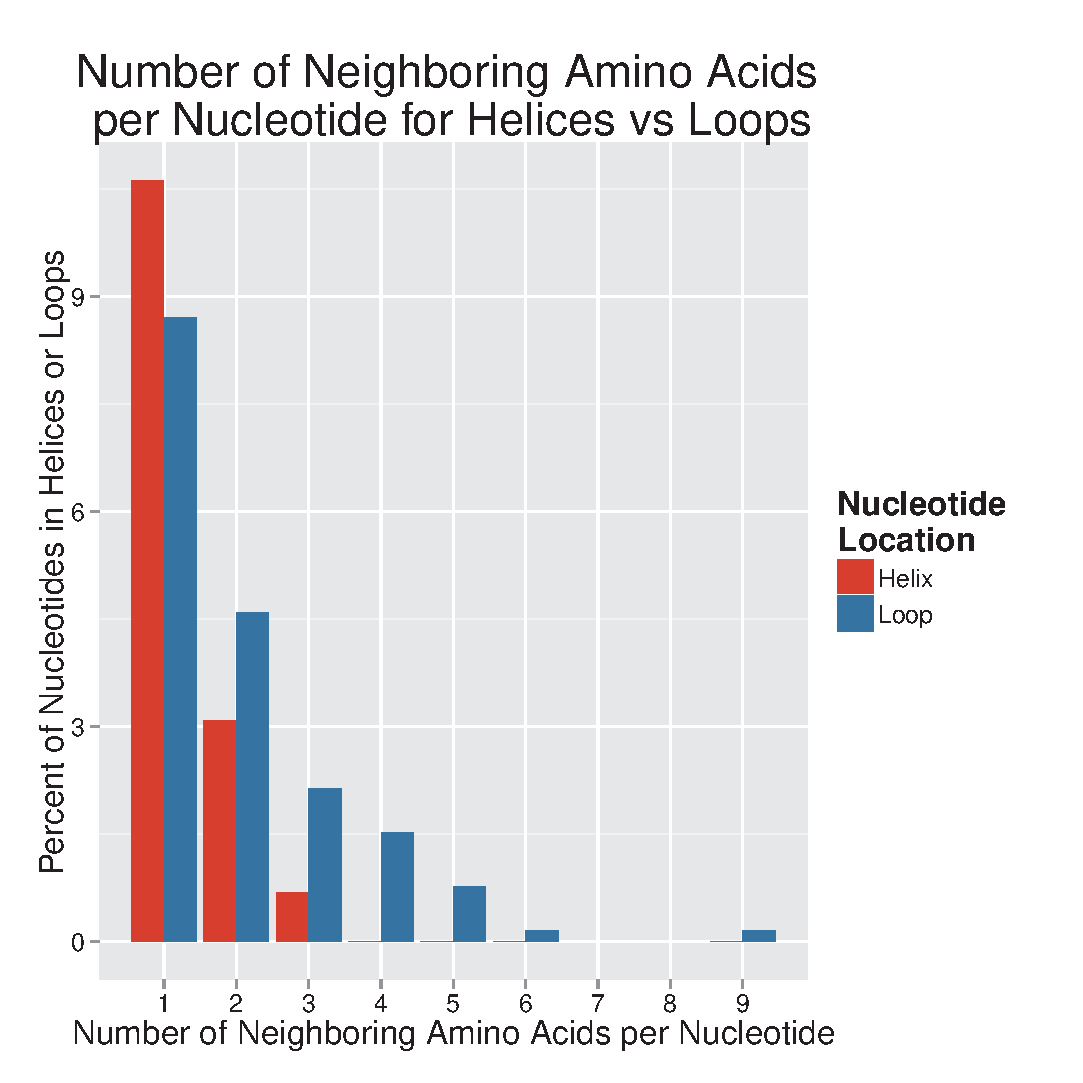
\includegraphics[width=0.5\linewidth]{chapter-1/figs/aa-loop-v-nt}
  \caption{Amino Acid Interactions for Loop vs. Helix Nucleotides. Histogram of
    number of amino acids within 4Å for nucleotides in loops (blue) vs helices
  (red) in E. coli 30S ribosome. }
  \label{fig:aa-loop-v-nt}
\end{figure}

The 30S particle also interacts with the large (50S) ribosomal subunit, or LSU,
to form the functional 70S ribosome. Non-covalent interactions or ``bridges''
that form between the subunits, many of which involve RNA, stabilize the
assembled 70S ribosome \cite{Yusupov2001}. Most of the 16S nts interacting with
the LSU are loop nts or helix nts adjacent to loops. 

About thirteen of the approximately 58 ``bulged out'' nts that do not interact
with other nts in \EC{} 16S rRNA, interact with SSU protein molecules. From
structures that contain bound mRNA and tRNA we observe that three others
interact with tRNA, three with mRNA, and A532, which is bulged out in 2AW7,
forms a bridge to the head domain of 16S when the head clamps down on the mRNAs
and the tRNA bound to the 16S A-site. Another bulged base, U723 forms a
base-phosphate interaction with the mRNA-Shine-Delgarno helix. A702, which
bulges out of the H23 kink-turn, interacts with 23S rRNA. Five others of these
58 ``looped out'' bases form perpendicular base-base interactions and eight form
base-ribose interactions. In summary only about half of the 58 nts (less than
thirty) are truly bulged out and of these \textasciitilde 21 facilitate tight turns in the 16S
backbone, of which 7 are in UNCG loops. 

The conclusion of this overview of the prevalence and roles of loop nts,
exemplified by 16S rRNA, is that almost all nts, whether they belong to ``loops,''
linkers, or helices in the 2D structure, form some kind of pairing, stacking or
base-backbone interactions. Moreover, interactions of loop nts constitute most
of the crucial long-range pairing, stacking and base-phosphate interactions that
stabilize domain structures and architectures and mediate most interactions with
proteins and other RNAs. Most of the very small number of truly “looped out”
bases play a role in facilitating formation of sharp \textasciitilde 180\degree turns in the RNA
backbone. 

For completeness, we conclude this section by briefly explaining the criteria
used to assign nts to helices and loops in a consistent way that can be applied
to analyze other structures and to automatically extract loop motifs for
detailed comparison and analysis.  This will help readers better understand how
motifs are extracted from structures for the RNA 3D Motif Atlas \cite{Petrov2013}, now
accessible through the revised NDB website \cite{CoimbatoreNarayanan2014}. 

\subsection{Assigning nts to helices and loops in structured RNAs}

While it is usually clear from accurate 2D diagrams, drawn with reference to 3D
data, whether a given nt should be assigned to the 2D structure, or to linkers,
HL, IL or MHJ loops, there are ambiguous cases that require clear definitions to
obtain consistent assignments. First, the choice of which helices to count as
Pseudoknots (PK) and which as part of the 2° structure is to some degree
arbitrary and different choices will also change the number of HL, IL, MHJ
loops, and linker regions \cite{Smit2008}. For example, if helix 2 (formed by
interactions between nts in the HL of helix 1 and the linker joining helices 27
and 28) is included in the 16S 2D, then H1 becomes the PK and a new 4-way
junction is defined, comprising H2, H3, H19 and H27. To build a comprehensive
Motif Atlas, it may be necessary, for each 3D structure, to cycle systematically
through alternative PK definitions to identify all motifs. Generally, the helix
formed by nts closest in the primary sequence is given precedence. Following
this guideline, helix 1 is favored over helix 2 for inclusion in the 2D. 

Second, there may be structural differences between PDB/NDB files for the same
RNA molecule. These differences can be due to inconsistencies or errors in the
3D modeling \cite{Stombaugh2009}, or to bona fide structural changes that occur
upon binding of substrates or other ligands. Furthermore, some regions of RNA
molecules are so dynamic that it is not possible to build unique
atomic-resolution models for them. In these cases, the structure must be
inferred by combining other data, including CSA, 3D modeling and structural
studies of RNA fragments. 

Even where all 3D structural models agree, further questions arise regarding how
to partition structures into helices and loops, including:

\begin{enumerate}
  \item Should single (isolated) Watson-Crick pairs that occur between two loops
    be assigned to the loops or to the 2D structure? 

  \item Should GU ``wobble'' pairs always be assigned to the 2D regardless where
    they are located? 

  \item How should other cis Watson-Crick pairs (AA, AC, AG, CC, CU and UU) be
    treated, especially when these form interfaces between helices and loops? 
\end{enumerate}

\subsubsection{Isolated Watson-Crick pairs}

Not infrequently, a single WC pair separates two loops. In which cases should
the WC pair be assigned to one of the adjacent loops and when should it be
considered part of the 2D structure? Alternatively, should the loops be merged
into a single 3D motif and the WC pair treated as belonging to this larger
motif? Examples of such “isolated” Watson-Crick base pairs in 16S rRNA occur
between IL in H17 and in H44 and between IL and MHJ loops in H5, H19, H22, H23,
H33, H40, and H42. 

The solution we propose is to treat loops separated by single WC pairs as
separate 3D motifs and assign the WC pair to the 2D, unless the nts of this WC
pair form extensive interactions with nts of each of the adjacent loops. In the
case of the H17 and H44, the interactions of the WC pairs are limited to base
stacking with neighboring bases in the sequence. In these cases the sequence of
the WC pair is less likely to be conserved and typical WC co-variation is
usually observed, and the adjacent loops are best treated as distinct motifs
with the WC pairs assigned to the 2D structure. However in the case of IL
adjacent to five of the MHJ loops of 16S rRNA there are additional interactions
involving the embedded WC pairs. Moreover, these pairs tend to be highly
conserved in sequence, due to the additional interactions. In these cases we
propose that the WC pair should be assigned to the MHJ loop and not to the 2D
structure. This was done in constructing Table 1. All the WC pairs marked with
red lines in Figure~\ref{fig:ec-ssu-2d-3d}  are of this type. 

\subsubsection{GU cWW pairs}

Sequence analysis shows that most cWW GU pairs in an RNA structure co-vary with
AU, UA, GC, and CG in homologous sequences, indicating that at these positions
GU pairs are functionally indistinguishable from WC pairs. Therefore we assign
cWW GU pairs that are adjacent to HL, IL, or MHJ loop motifs to the 2D
structure, just as is done for AU and GC pairs. This is the approach taken in
the construction of the 3D Motif Atlas \cite{Petrov2013}. Nonetheless, readers
should note that sequence analysis shows that highly conserved cWW GU base pairs
flank some HL, IL and MHJ loop motifs and perhaps these should be considered
parts of these motifs, at least operationally, for example, in designing
self-assembling RNA molecules for RNA nanotechnology or in 3D structure
prediction. This is an area of current research that requires integration of
comparative sequence analysis and biophysical characterization. In fact, in a
number of 3D motifs, exemplified by C-loops, the flanking WC pairs actually form
base triples with the loop nts, and therefore could be considered part of the
motif \cite{Lescoute2005}. Even though the RNA 3D Motif Atlas extracts each loop
motif together with its flanking Watson-Crick pairs to facilitate analysis of
their interactions and their sequence variations, the flanking WC pairs are
still considered part of the 2D structure \cite{Petrov2013}. 

\subsubsection{AG, AC and other cWW pairs}

AG \emph{cis} Watson-Crick (cWW) pairs are not uncommon in structured RNAs; they
tend to occur at the ends of helices flanking loop motifs, especially MHJ motifs
[27]. They rarely occur within helices because they are larger than AU or GC WC
pairs and therefore not isosteric to them, and when substituted for them,
distort the local helical geometry and destabilize adjacent WC base pairs.
Because cWW AG pairs almost always occur adjacent to loops and rarely co-vary
with GC or AU, we assign all cWW GA pairs to the loops rather than the adjacent
helices, consistent with the way they are treated in the 3D Motif Atlas. For
consistency, other non-WC cWW base pairs, including AC, AA, UU, CU, and CC, are
also treated this way.

In the next section we describe the components of RNA nucleotides to provide a
basis for understanding nucleotide-level interactions in RNA. 

\section{Components of RNA nucleotides}

The nucleotide is the basic unit of RNA structure. It is also the synthetic unit
or “synthon” from which RNA is produced in vivo. Each nucleotide is made of one
of the four RNA bases, Adenine (A), Cytosine (C), Guanine (G), or Uracil (U),
attached to ribose, a 5-membered sugar ring, which in turn is linked to one or
more phosphate groups. 

Two features distinguish RNA from DNA and have important structural
implications: the substitution of -OH at the 2'-carbon of the ribose ring in RNA
in place of -H in the deoxy-ribose ring of DNA, and the substitution of uracil
(U) in RNA for thymidine (T) in DNA. The 2’-OH facilitates H-bonding along the
``Sugar-edge'' of each RNA nt. U lacks the 5-methyl group of Thymidine (T),
located on the Hoogsteen edge of T; consequently U, but not T, can form base
pairs along its Hoogsteen edge. These structural differences make RNA more
versatile than DNA in forming interactions that support complex structures.

\subsection{Bases and Base Edges}

Each base is a nitrogen-rich, heterocyclic aromatic ring system that is planar
in its equilibrium geometry and quite rigid, due to delocalization of
pi-electrons. RNA bases are of two types, the pyrimidines (U and C), composed of
one six-membered aromatic, heterocyclic ring, and the larger purines (A and G),
composed of fused five- and six-membered rings. Structures of nts with the
numbering of base positions are shown in Figure~\ref{fig:bases}. Base ring atoms are numbered
from 1 to 9 in purines and from 1 to 6 in pyrimidines. Exocyclic groups and
attached hydrogen atoms are numbered according to ring position. Ribose atoms
are numbered with primes, from 1' to 5', to distinguish their atoms from those
of the base. 

\begin{figure}[p]
  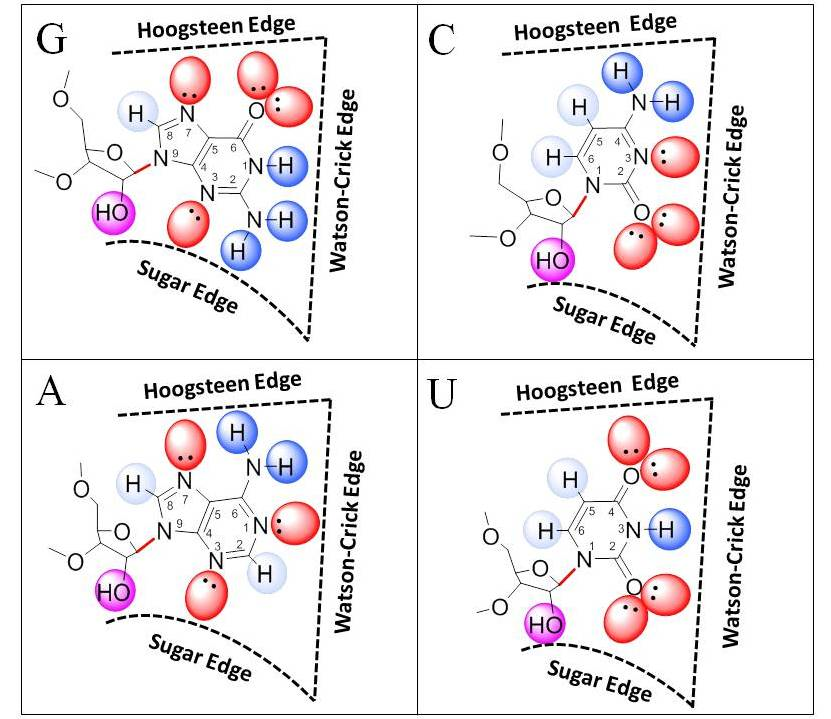
\includegraphics[width=\linewidth]{chapter-1/figs/bases}
  \caption{Structures of RNA nucleotides. RNA nts G, C, A, and U each have three
    edges along which H-bonding takes place. Hoogsteen, Watson-Crick, and Sugar
    Edges are marked with dotted lines. Base ring atoms are numbered from 1 to 9
    for purines and 1 to 6 for pyrimidines. Exocyclic groups and attached
    hydrogens are numbered according to ring position. H-bond donors are
  highlighted with blue and H-bond acceptors with red.}
  \label{fig:bases}
\end{figure}

The planar RNA bases present three ``edges'' studded with H-bonding donor and 
acceptor groups along which H-bonds can form with the edges of other bases, as
well as with phosphate and ribose groups, amino acid side chains or backbone
atoms of proteins and small molecules. These edges are called the Watson-Crick
(W), Hoogsteen (H) and Sugar (S) edges \cite{Leontis2001}. Therefore it is
useful to represent RNA bases, purines as well as pyrimidines, as triangles, or
more precisely, oblate triangular prisms to describe and classify their diverse
interactions as observed in RNA 3D structures \cite{Hoehndorf2011}. The base
edges are indicated for each RNA base in Figure~\ref{fig:bases}. Further support for
representing bases as triangles comes from the observation that bases can pair
edge-to-edge with up to three other bases at the same time, but no more than
three \cite{AbuAlmakarem2012b}. This explains the observation that no nt in 16S
forms more than three base pairs (see Figure~\ref{fig:ec-bp-loop-v-helix}). 

In triangles representing the RNA bases, two of the vertices coincide with
exocyclic H-bonding functional groups. The H and W edges meet at the vertex
defined by the N4 or N6 amino groups of C and A, respectively. The corresponding
atoms for U and G are the O4 and O6 carbonyl oxygen atoms. The W and S edges
meet at the vertex defined by the O2 carbonyl group in C and U, the polarized
C2-H2 of A, and the N2 amino group of G. The glycosidic bond connecting each
base to the C1’ carbon of the ribose defines the third vertex of the triangle,
where the H and S edges meet. The 2'-OH group, unique to RNA, extends the
H-bonding capability of the Sugar edge of each nucleotide

The RNA bases are shown in Figure~\ref{fig:bases} with H-bond donor groups
shaded with blue ``clouds'' and the H-bond acceptor groups shaded with red
``clouds,'' representing centers of positive and negative charge, respectively.
The ribose 2'-OH group is shaded in purple because it can serve as either H-bond
donor or H-bond acceptor. 

\subsection{Ribose sugar rings}

RNA bases are covalently attached to the 1'-carbons of their respective ribose
rings by single C-N bonds, the ``beta-glycosidic'' bonds. In the beta
configuration, each base is attached by the glycosidic bond to the same side of
its ribose ring as the ribose 5'-carbon atom. The ribose ring is a five-carbon
aldose sugar present in the furanose form. The flexible beta-glycosidic bonds
allow for relatively free rotation of the RNA base relative to the ribose
moiety. Rotation of the base gives rise to two distinct conformational classes
of the nucleotide, called anti and syn \cite{Neidle2008}. In the anti
configuration the Watson-Crick edges of the bases point away from the
5’-phosphate group. In the syn configuration the base is rotated \textasciitilde 180\degree
about the glycosidic bond so the WC edge faces the 5'-phosphate. G is the base
that is most often observed in syn. In the syn configuration, the N2 amino group
of G can H-bond to a 5'-phosphate oxygen atom. However, in polynucleotides, the
anti configuration is much more common. The anti configuration is stabilized by
weak H-bonding of the purine H8 or pyrimidine H6 atoms on the Hoogsteen edge to
the 5'-phosphate group. Whether a base is syn or anti affects the kinds of base
pairs it can form with nearby bases. One of the most common discrepancies
between published RNA 3D structures of the same molecule is the glycosidic bond
configuration of certain nts \cite{Leontis2002f}. 

\subsection{Phosphate groups}

Phosphate groups are derived from phosphoric acid (\ce{H3PO4}), a weak acid with
three dissociable protons that can form up to three phospho-ester linkages. In
RNA and DNA, there is one phosphate per base-sugar unit (``nucleoside'') and
each phosphate links two nucleosides, by forming two phospho-ester bonds. Each
phosphate is arbitrarily assigned to the nt to which it is attached at the
5’-hydroxyl group. The phosphate groups link adjacent nucleoside units to each
other by forming second linkages to the 3'-hydroxyls of the preceding one in the
linear chain. To link two nucleosides together, each phosphate loses two protons
(\ce{H+}) and forms two electrically neutral phospho-ester linkages. The
remaining proton is acidic and largely dissociates at neutral pH. Therefore each
phosphate group in RNA carries a full negative (-1) electrical charge, which is
delocalized over the two non-bridging oxygen atoms of the phosphate group,
making them strong H-bond acceptors. Consequently, base-phosphate interactions
play structurally important roles and can be as stabilizing as GC base pairs
\cite{Zirbel2009, Sponer2010}. Large RNA molecules like 16S rRNA, therefore,
have substantial negative charge that must be neutralized by H-bonding
interactions or mobile positive ions in order for the RNA to fold into its
functional structure. In vivo, charge neutralization depends on \ce{Mg2+},
assisted by basic proteins and polyamines \cite{Draper2008}.

\subsection{RNA Backbone Conformations}

The backbone of the RNA chain is very flexible and able to assume many different
conformations because each nt contributes six covalent single bonds, including
the C3'-C4' and C4'-C5' bonds of the ribose ring and two C-O and O-P bonds
comprising the two phospho-ester linkages. The conformation of each nt is
defined by the set of values of the dihedral angles of these bonds together with
that of the glycosidic bond \cite{Neidle2008}. The dihedral angles of each Nt
are assigned Greek letters, alpha ($\alpha$) to zeta ($\zeta$), starting with
the P-O5' bond of the 5'-phosphate and continuing consecutively with the
O5'-C5', C5'-C4', C4'-C3', C3'-O3', and ending with the O3'-P bond of the
3'-phosphate. The glycosidic bond (``chi'' or $\chi$) contributes the seventh
dihedral angle. These seven dihedral angles define a very large,
seven-dimensional conformational space for each nucleotide. However there are
extensive correlations between the values of the dihedral angles, so that
relatively few regions of this seven-dimensional space are populated to a
significant extent in observed or theoretically possible structures. It is most
convenient to cluster conformations by parsing the RNA backbone in overlapping
``suites'' that extend from one sugar to the next, rather than from one
phosphate group to the next \cite{Richardson2008}. Analysis of atomic-resolution
experimental data using this approach enabled researchers to determine that the
backbone conformations of structured RNA molecules are ``rotameric''
\cite{Murray2003}. In other words, most observed conformations can be grouped in
well-defined clusters of conformations, many of which are characteristic of
particular structural motifs. This analysis identified 42 recurrent rotamer
clusters in RNA structures, each of which was assigned a two-symbol
representation \cite{Richardson2008}. While the experimental data are still
incomplete and we can expect to discover additional energetically accessible
conformations or rotamers, these are likely to be rare or similar to ones
already reported. Conformational analysis of each suite in each structure is now
a standard reporting function of NDB \cite{CoimbatoreNarayanan2014}. 

As many conformations have similar energies, the selection of local nt
conformations as RNA molecules fold is guided largely by the specific
interactions formed by the bases, especially base-pairing. We turn to these
next. 

\section{Nucleotide interactions}

For an RNA chain to fold into a distinct 3D structure, the nucleotides must form
specific and energetically favorable non-covalent contacts. RNA nucleotides can
interact with each other in many different ways. These can be broadly classified
as 1) base with base, 2) base with ribose sugar, 3) base with phosphate, 4)
ribose with ribose, 5) ribose with phosphate, and 6) phosphate with phosphate. 

We begin with base-base interactions and then consider base-phosphate and
base-sugar interactions. Base-base interactions are the most sequence specific,
and therefore the most useful for predicting RNA structures or designing RNA
sequences to fold in desired ways for RNA nanotechnology applications.
Base-phosphate and base-ribose interactions are base specific for one of the two
interacting nucleotides. Ribose-ribose, ribose-phosphate and phosphate-phosphate
interactions are not sequence-specific and consequently difficult to classify
informatively for RNA prediction and design, and will not be discussed further.
Nonetheless, all these interactions contribute to the energetics of RNA folding
and we can expect that analysis of their local contexts, recurrent geometries,
and relative frequencies will prove valuable in the evaluation of de novo
modeled and predicted 3D RNA structures. Although the negatively charged
phosphate groups repel each other, precluding direct contact, the phosphates can
indirectly interact through bridging divalent ions, especially \ce{Mg2+}, which is
maintained at milli-molar (mM) concentration in cells. Metal-bridging
interactions are very important for the compact folding of complex RNA
architectures and have been reviewed elsewhere cite{Woodson2005, Bowman2012}. 

\subsection{Base-Base Interactions}

RNA bases interact with each other primarily by edge-to-edge H-bonding
(``base-pairing'') and by face-to-face van der Waals bonding
(``base-stacking''). In principle, bases can also interact edge-to-face
(``perpendicular interactions''). In crystals of aromatic hydrocarbons
compounds, perpendicular interactions are frequently observed
\cite{Desiraju1989}. Perpendicular interactions can be found in RNA 3D
structures using the FR3D motif search program \cite{Petrov2011a}. Although
relatively rare, they deserve to be studied systematically to determine
recurrent geometries and sequence propensities. 

\subsubsection{Base-pairing Interactions}

Base pairing results from H-bonding interactions between the edges of two RNA
bases, a consequence of the geometric regularities of the RNA bases and the
presence of at least two H-bond donor or acceptor groups on each base edge.
H-bonds are attractive electrostatic interactions between H-atoms covalently
bonded to highly electronegative atoms, primarily O and N in biomolecules, and
electronegative atoms bearing unpaired electrons, also O or N for the most part.
Individual H-bonds are highly directional but relatively weak non-covalent
interactions. Therefore, stable association between the edges of two bases
generally requires forming two or more H-bonds. Specificity is achieved because
H-bonds are directional and require juxtaposition of complementary donors and
acceptors, as exemplified by the H-bonding between the Watson-Crick edges of G
and C or A and U to form canonical Watson-Crick base pairs. 

RNA bases can form many types of base pairs, in addition to the well-known WC
pairs, because they have three distinct edges available for H-bonding
\cite{Leontis2001, Leontis2002f}, the Watson-Crick edge (W), the Hoogsteen edge
(H) and the Sugar edge (S) as shown in Figure~\ref{fig:bases}. The base edges
interact with each other in all combinations, W with W, W with H, W with S, H
with H, H with S, and S with S, and in each of two orientations, cis and trans,
to create twelve geometrically distinct types of base pairs \cite{Leontis2001}.
These twelve types of base pairing geometries are shown schematically in Table 3
using right triangles to represent RNA bases. The Hoogsteen edge corresponds to
the hypotenuse of each triangle in Table 3 and the marked vertex indicates the
location of the ribose sugar. 

Table 3 also shows symbols developed to mark base pairs in extended 2D diagrams.
In these symbols, circles represent Watson-Crick edges, squares Hoogsteen edges
and triangles Sugar edges. Base pairs involving distinct edges are represented
by two symbols connected by a line. For example, a trans Watson-Crick/Hoogsteen
base pair (tWH) is represented with a circle linked to a square. The symbol is
placed in 2D diagrams so that the circle faces the letter representing the base
bonding with its W edge and the square the base bonding with its H edge. When
both bases use the same edge to form the pair, a single symbol suffices. Filled
symbols represent cis base pairs and open symbols trans base pairs. Annotating
2D diagrams in this way conveys crucial 3D interaction information to readers,
at least for local interactions. Representing all long-range interactions
observed in the 3D structure is more difficult because the 2D diagram can become
very cluttered with symbols if these are not drawn carefully. 

\subsubsection{Exploring non-WC Base pairing}

Within each base pair family different base combinations (A with U, G with C, U
with U, etc.) can form geometrically similar base pairs, depending on the
arrangement of H-bond donor and acceptor groups on each base edge. To help the
reader explore the base-pairing possibilities of RNA bases, we have prepared
planar structures of the four nucleotides that can be xeroxed onto colored
transparencies and cut out individually (see Figures \ref{fig:ua} and
\ref{fig:gc}). Each nt is reproduced in two distinct orientations, to aid in
forming cis as well as trans base pairs. Possible base pairs can be explored by
aligning base edges in various combinations to identify potentially stable
H-bonding arrangements. To guide the reader in this exercise, lone pair
electrons have been included on the exocyclic carbonyl oxygen and ring imine
nitrogen atoms; these serve as electron-rich, H-bond acceptors and are colored
red. Readers will note that the lone pairs of exocyclic amino groups (GN2, CN6,
and AN6) are not shown in these diagrams because these electrons are delocalized
into the aromatic rings and are generally not available as H-bond acceptors,
except in special cases \cite{Zirbel2009, Sponer2003}.

\begin{figure}
  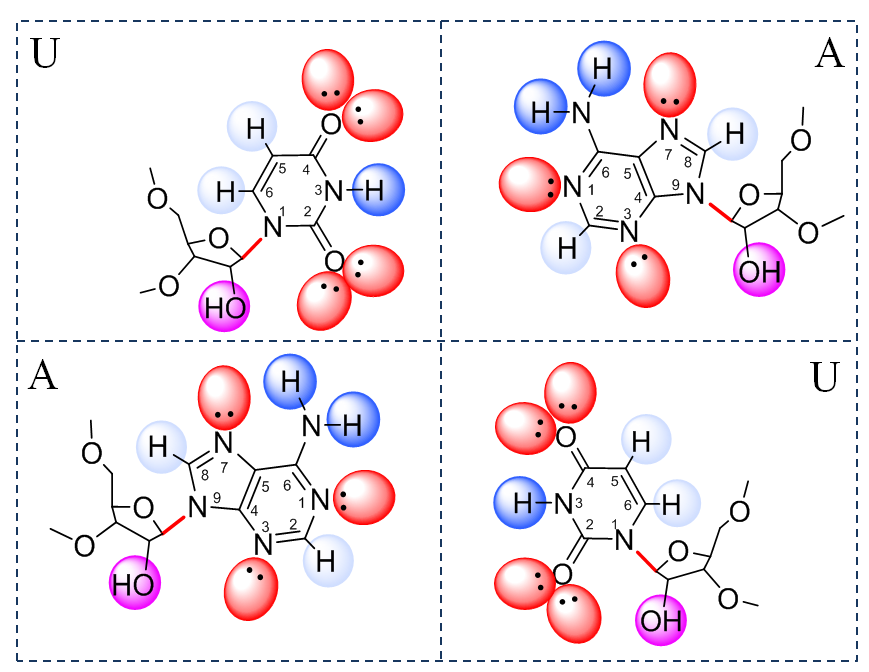
\includegraphics[width=\linewidth]{chapter-1/figs/ua}
  \caption{U and A Nucleotides to print on transparencies. U and A nts in two
    orientations to print on transparencies for making base pairs by juxtaposing
  H-bonding donor (blue) and acceptor (red) groups. }
  \label{fig:ua}
\end{figure}

\begin{figure}
  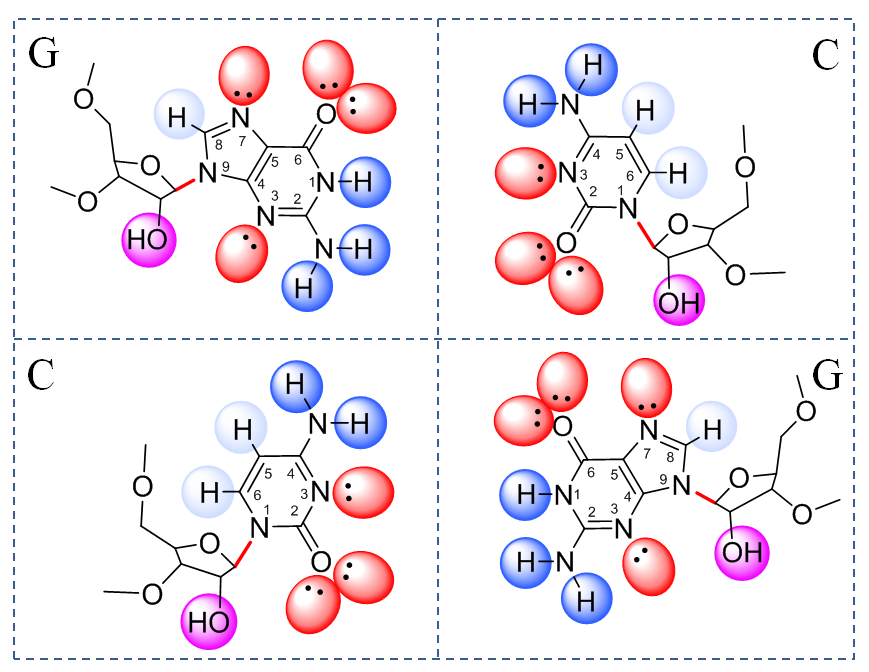
\includegraphics[width=\linewidth]{chapter-1/figs/gc}
  \caption{G and C Nucleotides to print on transparencies. U and A nts in two
    orientations to print on transparencies for making base pairs by juxtaposing
  H-bonding donor (blue) and acceptor (red) groups.}
  \label{fig:gc}
\end{figure}

The H-bond acceptor groups are colored red in Figures \ref{fig:ua} and
\ref{fig:gc}, to reflect their overall negative charge. H-bond donor groups,
comprising H-atoms covalently bonded to electro-negative oxygen or nitrogen
atoms, are colored blue, reflecting their overall positive charges. The goal
when manipulating the colored transparencies is to obtain stable base pairs by
juxtaposing H-bond donors and acceptors so as to form at least two H-bonds. Each
red-colored functional group should partly overlap a blue-colored functional
group while avoiding any red-with-red or blue-with-blue juxtaposition. The 2’-OH
(hydroxyl) groups are colored purple to indicate that they can serve either as
H-bond donors or acceptors. Moreover, a single hydroxyl group can simultaneously
interact with an H-bond acceptor and at least one H-bond donor. The –OH bond can
rotate as needed to optimize H-bonding.

\begin{figure}
  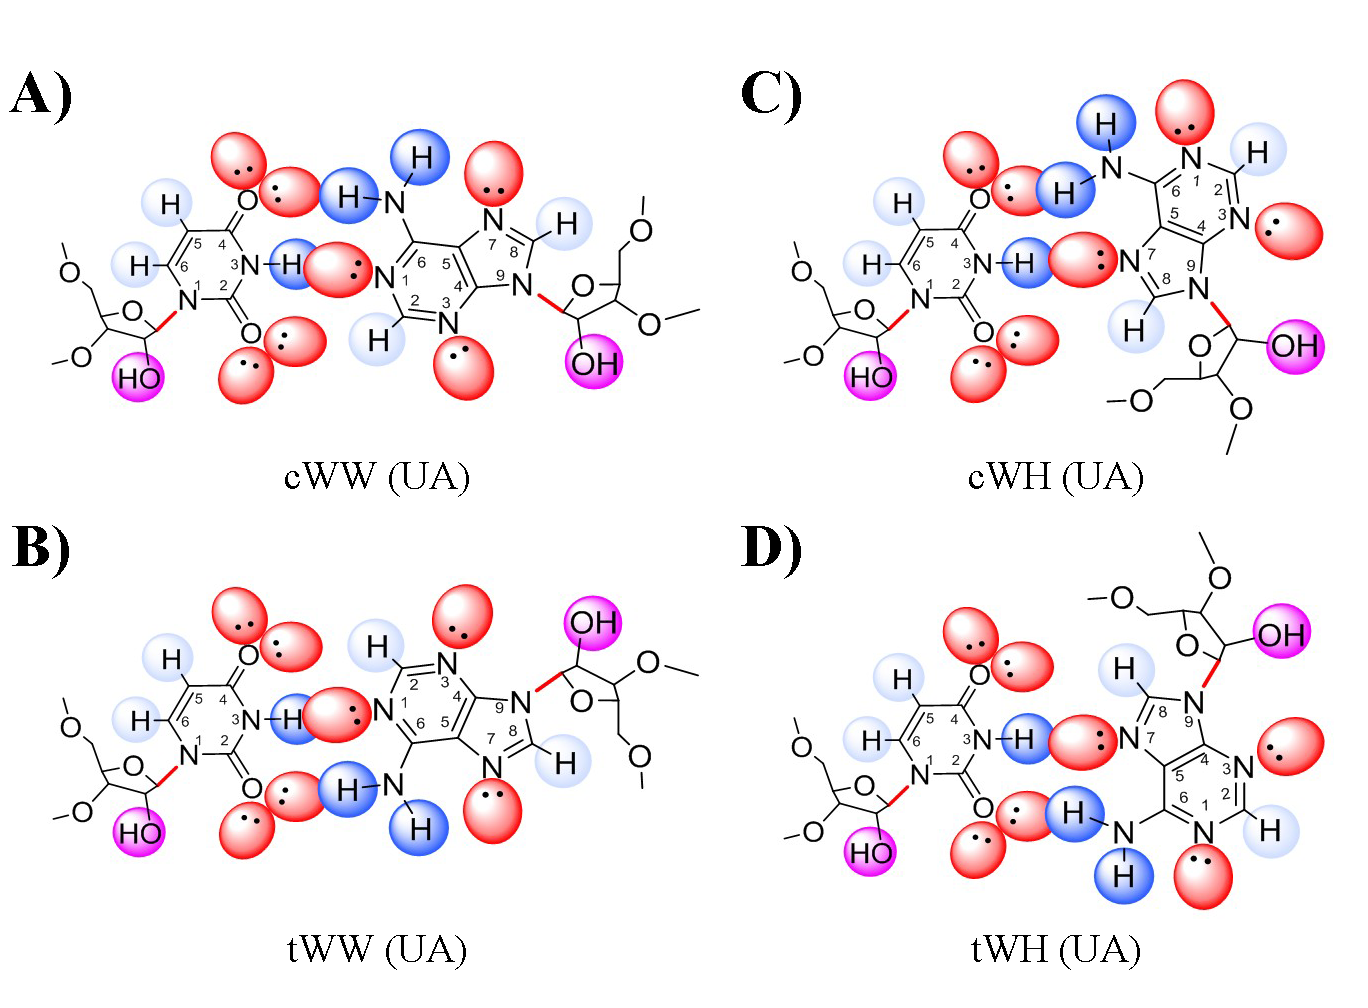
\includegraphics[width=\linewidth]{chapter-1/figs/basepairs}
  \caption{Representative basepairs. UA base combination in four different
    basepairing geometries: A. \emph{cis} Watson-Crick/Watson-Crick (cWW); B. \emph{trans}
    Watson-Crick/Watson-Crick (tWW); C. \emph{cis} Watson-Crick/Hoogsteen (cWH); and D.
  \emph{trans} Watson-Crick/ Hoogsteen (cWH).}
  \label{fig:basepairs}
\end{figure}

To get started, readers can arrange the transparent cutouts of uracil and
adenine having WC edges facing in opposite directions to form the canonical AU
cis Watson-Crick (cWW) base pair. This pair is shown in Figure~\ref{fig:basepairs}A to illustrate
the complementary arrangements of color-coded H-bond donating and accepting
groups, red opposite blue. The H-atom attached to C2 of adenine (AH2) is colored
light blue to show that it is slightly polarized and capable of weak H-bonding
with O2 of uracil. Other H atoms covalently bonded to carbon atoms that are
sufficiently polarized to form weak H-bonds are also colored light blue. 

To form the non-WC trans Watson-Crick (tWW) UA pair, the A and U cutouts printed
with W edges facing in the same direction can be used.  Bringing together the W
edges forms an AU trans Watson-Crick (tWW) base pair, that can be compared with
Figure~\ref{fig:basepairs}B. This pair differs from the canonical (cis) Watson-Crick AU base pair
in the mutual orientation of the glycosidic bonds. In the cis pair, the
glycosidic bonds are on the same side of the base pair axis running through the
base centers parallel to the H-bonds, while in the trans pair, the glycosidic
bonds are on opposite sides of this axis.  

Next readers can reorient the W edge of the U so that it faces the H edge of the
A, juxtaposing complementary H-bond donor and acceptor groups. Results can be
compared with the pairs shown in Figure \ref{fig:basepairs}C and
\ref{fig:basepairs}D. There are two possible results, the \emph{cis} and the
\emph{trans} Watson-Crick/Hoogsteen pairings (cWH or tWH UA). These pairs are
stabilized by two strong H-bonds, involving NH donors, and one relatively weak
bond involving AH8. These base pairs have the same base combination (UA) as the
cWW and tWW pairs, but involve the Hoogsteen edge of A, illustrating that each
distinct combination of edges and glycosidic bond orientations produces a
different base-pairing geometry and therefore a different pair. 

Readers are encouraged to try other base combinations, to see how many form
stable pairs for each geometric family, and can check their base-pair models
against the on-line RNA Base pair Catalogue containing structures of all
observed and predicted base pairs organized by geometric family
(\url{http://rna.bgsu.edu/FR3D/base pairs/}). The base combinations that form
pairs in each pairing geometry are summarized in Table 4.

\subsubsection{The Sugar Edge}

A key concept for understanding sugar-edge base pairing is the role of the
ribose 2’-OH group, which can serve as an H-bond donor or acceptor, and often,
both simultaneously, on account of the free rotation of the hydroxyl group about
the C2’-O2’ single bond and the presence of the non-bonding electron orbitals on
the oxygen. Consequently, many different pairs can form using the sugar edges of
nts.  

\subsubsection{Protonation of the Watson-Crick edge of A and C}

Another important concept is that the imine nitrogen atoms, AN1 and CN3, on the
Watson-Crick edges of A and C, which are normally unprotonated and act as H-bond
acceptors, can be protonated at a modest energetic cost, when required by the
context, to convert these groups to H-bond donors. This allows certain base
combinations to form base pairs that cannot form when A or C are in their
unprotonated forms. Protonation confers a positive charge to the resulting BP,
which can help stabilize accumulations of negative charge, as occur, for example
in the close packing of phosphate groups or during chemical reactions
\cite{Siegfried2010, Cerrone-Szakal2008a}. Allowing for H-bonding to 2'-OH and
protonation of A and C Watson-Crick edges expands the number of base pairs one
can construct. 

\subsubsection{Specifying non-WC Base Pairs: Base combinations and Base-pair
families}

As readers experiment with the RNA base cut outs to construct base pairs, they
will quickly discover that the same base combination, for example UA in the
examples above, can form several different types of base pairs. To keep track of
the base pairs that form, readers should note the geometric base pair type or
family, in addition to the base combination. Giving the interacting edges of the
bases and the relative orientations, cis or trans, of the glycosidic bonds,
specifies the base pair family. To specify individual pairs, both the base
combination and the base pair family are needed, for example, UA tWH, UA cWW, or
CG cWW. 

It is necessary to specify the base combination because in each base pair
family, different base combinations (up to sixteen) can form the same type of
base pair. For example, fifteen of the sixteen base combinations, all except GG,
can form cWW base pairs. The base combination AG can form eleven of the twelve
different types of base pairs, all families except tWW. Referring to non-WC base
pairs as ``mismatches,'' as is frequently done in the literature, is imprecise and
misleading because for stable non-WC, as for WC, pairings, at least two H-bonds
form between the interacting edges. The only ``mismatches'' are those base
combinations that cannot form a particular base pair type. For example, GG is a
``mismatch'' for cWW but a stable ``match'' for tWW. It is better to simply speak of
``allowed'' and ``non-allowed'' base combinations for each base pairing geometry. As
noted above, some base combinations require protonation to form. In such cases,
the energy penalty for protonation is compensated by the more favorable binding
energy.

Readers can check their base-pair models against the on-line RNA Base pair
Catalogue containing structures of all observed and predicted base pairs
organized by geometric family (\url{http://rna.bgsu.edu/FR3D/base pairs/}) and
by comparison with Table 4. The base combinations (columns of Table 4) that form
a stable pair in a particular base pair geometry (rows of Table 4) are indicated
with an entry beginning with ``I.'' If no stable pair forms for that geometry, the
cell is left empty. Each column shows the base pair geometries that each base
combination can adopt. The 3D structures of base combinations forming pairs in
each geometric family can be viewed and downloaded as PDB files from the pages
of the online Base Pair Catalogue. 

Regarding Table 4, readers should note that for base pair geometries that
involve different edges (for example cWH or tHS) the order in which the bases
are listed makes a difference. For example, in the tWH AG base pair, the A
interacts with its W edge and the G with its H edge. Consequently, ``AG tWH''
and ``GA tWH'' refer to different base pairs. On the other hand, ``tWH AG'' and
``GA tHW'' refer to the same base pair. However, tHW pairs do not have their own
row in Table 4 because they are redundant with tWH pairs. 

\subsection{Base pair Isostericity and Sequence Variation}

The classification of base pairs into geometric families based on edges provides
the framework for making sense of the base substitutions observed in structural
alignments of recurrent RNA 3D motifs and sequence alignments of RNA homologs
(for example, 16S rRNAs from different micro-organisms). To illustrate the basic
ideas, we first consider the AU, UA, GC, and CG Watson-Crick base pairs that
constitute the geometrically regular, anti-parallel double helices of RNA. RNA
helices are regular precisely because AU and GC pairs can substitute for each
other with little or no distortion of the helical geometry. They are said to be
isomorphic or “isosteric” to each other in the sense of occupying the same space
between the backbone atoms of the two strands of the helix. The property of
being isosteric can be quantified using a measure called the Iso-Discrepancy
Index (IDI), which depends on three distinct geometric features of base-pairs,
as illustrated in Figure~\ref{fig:idi} \cite{Stombaugh2009}. The geometric classification
of base pairs is useful because only base pairs belonging to the same family are
isosteric by qualitative and quantitative (i.e. the IDI) criteria. Isosteric
pairs substitute for each other without distorting the local RNA 3D structure.
The IDI was calibrated by carrying out statistical analysis of IDI values of
isosteric and near isosteric AU, GC, and GU base pairs extracted from
high-quality structures. Quantitative analysis with IDI values confirms that for
two base pairs to be isosteric, they must belong to the same geometric family
\cite{Stombaugh2009}. 

\begin{figure}
  \includegraphics[height=0.5\textheight]{chapter-1/figs/idi}
  \caption{Calculation of Iso-Discrepancy Index (IDI) to compare geometries of
    basepairs. The IDI is illustrated using non-isosteric base pairs. To
    calculate the IDI for two base pairs, the bases designated ‘first base’ in
    each base pair are superposed (bases on the left in each panel) and then the
    following three quantities are evaluated, normalized and summed: (1) The
    difference, ∆c, in the intra-base pair C1’–C1’ distances, illustrated for
    non-isosteric cWW AG and AU. (2) The inter-base pair C1’–C1’ distance, t1,
    between the C1’ atoms of the second bases of the base pairs, illustrated for
    the near isosteric cWW AU and AC base pairs. (3) The angle, theta, about an
    axis perpendicular to the base pair plane, required to superpose the second
  bases, illustrated using non-isosteric cWW AU and cWS AU base pairs.}
  \label{fig:idi}
\end{figure}

All base pairs from the same geometric family have equal or very similar values
of the angle describing the mutual orientations of the glycosidic bonds of the
interacting bases, however they can differ by the other geometric measures used
to define the IDI (see Figure~\ref{fig:idi}). Therefore, not all base pairs belonging to
the same geometric family are necessarily isosteric. For example, purines and
pyrimidines differ considerably in size, so substituting a purine by a
pyrimidine or vice versa may change the space occupied by the base pair within
its structural context, as measured by the distance between C1' atoms of the
interacting nts. For example, substituting A for C in a cWW CG base pair to
produce cWW AG significantly increases the C1'-C1' distance from \textasciitilde 10.4 \AA,
typical for AU or GC, to \textasciitilde 12.3 \AA. Consequently, this substitution distorts the
helix and destabilizes neighboring base pairs in the helix. Consistent with this
prediction, substitution of base combinations AG or GA for cWW CG or AU pairs
within regular helices of homologous RNA molecules is rare, and cWW AG pairs
occur almost exclusively on the ends of helices, often adjacent to junction
motifs where they provide a large surface for stabilizing inter-helix stacking
interactions \cite{Sponer2003}. An example is the cWW AG pair, found in most
tRNAs at the top of the anticodon stem-loop and flanking the tRNAs MHJ
\cite{Romby1985}.

To properly align the H-bond donor and acceptor groups of the substituted bases,
it may be necessary to shift the bases laterally relative to the positions of
the original bases. Such a shift is needed when U substitutes for C to transform
a GC to a GU cWW pair, so that the H-bond donor and acceptor groups on the
Watson-Crick edges of G and U can align. The U shifts laterally toward the major
(deep) groove, relative to the G, to form the GU pair. This geometric change is
not as disruptive to adjacent base pairs, as the changes in C1'-C1' distances
that occur with AG cWW pairs. Consequently, GU pairs are observed quite
frequently within Watson-Crick helices in RNA molecules. The cWW GU pair is
considered ``near isosteric'' to cWW GC and AU. However, the lateral shift breaks
the symmetry of the cWW geometry, so cWW GU and UG pairs are geometrically
distinct and not isosteric or even near isosteric to each other. In each base
pair family, different sets of base combinations form pairs that are isosteric
to each other. For example, the base combinations AG and CU are isosteric in the
tHS family although they are not isosteric in the cWW family \cite{Leontis2002f, Leontis1998b}.

These considerations predict that those base substitutions that result in
isosteric or near isosteric base pairs should be much more likely to occur
between homologous molecules than non-isosteric ones. The rRNAs of \EC{} and
\TT{} provide an ideal, large-scale test case for this hypothesis, because these
two bacteria are phylogenetically and ecologically divergent. Nonetheless, their
3D rRNA structures are sufficiently conserved that a large percentage of base
pairs in the two structures can be structurally aligned and compared
\cite{Stombaugh2009}. The base pairs of 5S, 16S, and 23S rRNAs from high quality
structures of 70S ribosomes of these species were aligned manually to identify
corresponding base pairs. It was found that over 90\% of base pairs could be
aligned and analyzed using the IDI. This analysis showed that 72\% of
corresponding base pairs in the 5S, 16S, and 23S rRNAs of \EC{} and \TT{} were
isosteric and unchanged in sequence, 19\% were isosteric and different in
sequence, 7\% were near isosteric, and only 2\% were non-isosteric
\cite{Stombaugh2009}. In total, almost 98\% of the alignable base pairs in the
two structures were isosteric or near isosteric. This results provides strong
support for the generalization that base substitutions in homologous RNA
molecules or recurrent structural motifs are constrained to preserve isosteric
base pairings, whether the pairings are WC or non-WC.

NDB provides annotations for base pairs and other nt interactions for all
atomic-resolution 3D structures [9]. The annotations are accessible from the
main page of each structure. 

\subsection{Base Triples}

Base triples are common sub-motifs in RNA 3D motifs. All base triples can be
decomposed into combinations of base pairs, in which a central base is paired to
each of the other two bases of the triple using a different base edge. All in
all there are 108 different geometric base triple families of which 68 have been
observed in experimental structures \cite{AbuAlmakarem2012b}. The base-pair
families to which a base triple's component base pairs belong define the base
triple family to which it belongs. A catalog of observed base triples can be
accessed online through NDB. New base triples can be found by symbolic search
using FR3D \cite{Petrov2011a}. 

\subsection{Base-Stacking Interactions}

The energetically most stabilizing contributions to RNA structure are provided
by the hydrophobic van der Waals forces mediating stacking of the faces of RNA
bases on each other \cite{Sponer2010}. Because RNA bases lack rotational
symmetry, the two faces are not equivalent. Therefore two RNA bases can stack
face-to-face in four distinct ways, depending on which base faces come into
contact. The faces are distinguished by reference to the orientation of each
base in the Watson–Crick helix, in which all bases are in the anti-glycosidic
conformation; the ``5′-face'' points toward the 5′-end of the strand and the
``3′-face'' points toward the 3′-end of the strand \cite{Hoehndorf2011,
Sarver2008a}. A systematic analysis of the sequence propensities of base
stacking in all possible geometries and contexts is still lacking. NDB provides
base-stacking annotations for all RNA structures which can be used as a basis
for such studies. 

\subsection{Base-backbone Interactions }

\subsubsection{BPh interactions}

As each nt bears a full negative electrical charge, RNA molecules need to
overcome electrostatic self-repulsion to achieve compact folding. The negative
charge of each nucleotide is largely concentrated on the two non-bridging oxygen
atoms of the phosphate groups, resulting in electrostatic repulsion between
phosphate groups but enhancement of H-bonding to donors on base edges of the RNA
bases.  The stabilizing H-bonding interactions between bases and the phosphate
backbone moieties, referred to as ``base-phosphate'' (BPh) interactions, help to
reduce intra-molecular repulsion between phosphate groups while specifically
stabilizing compactly folded structural motifs and architectures. The
classification of BPh interactions by base is shown in Figure 14. This
classification is the result of structural bioinformatics study combined with
quantum mechanical (QM) calculations and molecular dynamics simulation studies
\cite{Zirbel2009, Zgarbova2011a}. The QM calculations revealed the optimal
geometries and the intrinsic stabilizing energies of these interactions, and
showed that the most stable BPh interactions, those on the W edge of G, rival GC
WC base pairs in stability. Very stable BPh interactions also are formed by the
WC edge of U and the Hoogsteen edge of C (see Figure~\ref{fig:bph} and citation
\cite{Zirbel2009}).

\begin{figure}
  \includegraphics[width=\textwidth]{chapter-1/figs/bph}
  \caption{Base-Phosphate (BPh) interactions observed in RNA 3D structures for
    each base. H-bonds are indicated with dashed lines. BPh categories are
    numbered 0–9, starting at the H6 (pyrimidine) or H8 (purine) base positions.
    BPh interactions that involve equivalent functional groups on different
    bases are grouped together: 0BPh (A, C, G, U), 5BPh (G, U), 6BPh (A, C),
    7BPh (A, C) and 9BPh (C, U). Bridging interactions, 8BPh and 4BPh, are
  especially stable.}
  \label{fig:bph}
\end{figure}

Many recurrent 3D motifs contain specific BPh interactions that tend to be
highly conserved. For instance, many hairpin loops, including the anti-codon and
T-loops of tRNAs, contain the ‘U-turn' submotif, a sharp bend in the backbone
stabilized by H-bonding between the WC edge of U and the phosphate of the N+3
base of the loop \cite{Quigley1976} A conserved BPh interaction involving the
conserved ``bulged'' G is observed in recurrent sarcin-ricin (S/R) internal loop
motifs \cite{Correll1998}. Conserved GU wobble base pairs are observed to bind
anionic oxygen phosphate atoms in the minor groove to facilitate tight packing
of helical elements \cite{Mokdad2006b}. It is necessary to consider conserved
BPh interactions to fully account for the chemical protections observed in 16S
rRNA \cite{Merryman1999, Stern1988}. These examples show that BPh interactions
are widespread in RNA structures and play significant roles in RNA folding, as
documented in Table 2.

\subsubsection{Base-Ribose Interactions}

The 2'-OH of ribose participates in sugar-edge base pairs, acting as both H-bond
donor and acceptor. It is considered part of the nt Sugar edge. H-bonds can also
form with the ribose O4' atom, acting as H-bond donor. Another type of
interaction involves stacking of bases on ribose rings as shown in
Figure~\ref{fig:base-ribose}. The example in this figure is a key interaction
that stabilizes the binding of tRNAs to the P-site of the 30S subunit. The
base-ribose stacking occurs between the ribose of the first anti-codon nt of
tRNA (G34) in the anti-codon HL (nts 32-38 of tRNA) and the highly conserved
base G966, located in HL 34 of 16S rRNA (an intermolecular loop-loop
interaction). Because only the tRNA ribose and not the base is involved in the
interaction with 16S, the base can vary in sequence, allowing tRNAs with
different anti-codon sequences to bind to the same site. The 16S base involved
in the interaction, G966, on the other hand is highly conserved and is in fact
chemically modified \cite{Burakovsky2012}. The sequence propensities of
base-ribose stacking interactions also deserve attention. Annotations of
base-ribose interactions are also posted on NDB.

\begin{figure}
  \includegraphics[width=\textwidth]{chapter-1/figs/base-ribose}
  \caption{Base-ribose stacking interaction. The conserved base-ribose stacking
    interaction involving ribose 34 in the anti-codon of tRNA bound to the
    P-site of 16S rRNA and conserved base G966 in 16S.  From PDB file 4GD1
    \cite{Dunkle2011a}.}
  \label{fig:base-ribose}
\end{figure}

\subsubsection{Metal-ion mediated phosphate-phosphate interactions}

Structured RNA molecules generally require multi-valent metal ions to fold into
their compact, functional structures \cite{Woodson2005, Bowman2012, Draper2005,
Draper2013, Auffinger2011, Tan2011}. This is because cations like \ce{Mg2+} can
bridge between two or more negatively charged phosphate groups, allowing compact
structures to form in which phosphate groups are in close proximity. Cationic
polyamines and basic proteins can also promote RNA folding \cite{Klein2004a,
Koculi2006}. \ce{Mg2+} is particularly well suited to facilitate rRNA compaction
because it is abundant in cells and has a very high charge density among
biologically available ions, owing to its relatively small ionic radius (0.6\AA)
and +2 electrical charge. \ce{Mg2+} associates preferentially with the anionic
non-bridging oxygen atoms of the phosphate groups. 

\subsection{RNA 3D motifs and non-WC pairs}

Recurrent modular 3D motifs generally correspond to individual HL, IL, or MHJ
loops. As we have seen, ``loops'' play very important roles in structured RNA
molecules. While some motifs appear to be unique, many occur over and over in
unrelated RNA molecules. Most recurrent 3D motifs are relatively small (less
than \textasciitilde 20 nts) and therefore can evolve independently in unrelated molecules.
For example, kink-turns, sarcin-ricin motifs, C-loops, and GNRA or UNCG HL are
found in many different molecules and even in multiple locations in the same
large RNA molecule. In fact, 16S rRNA contains instances of each of these
motifs. Non-WC pairs play two fundamental roles in RNA 3D structure: (1) They
are the building blocks of RNA 3D motifs \cite{Leontis2006}, where they provide
the specific local interactions that structure individual HL, IL and MHJ 3D
motifs. (2) Non-WC pairs mediate most LR (tertiary) interactions, usually in
combination with LR WC pairs, base-stacking, and base-phosphate interactions, as
discussed above for 16S rRNA. As we have seen, most of these interactions occur
between loop nts or loop and helix nts. The different types of non-WC pairs tend
to contribute to different extents to local vs. LR interactions, as shown in
Table 5. For example, cWW, tWH, and tHS together account for almost 90\% of
local base pairs, whereas cSS, tSS, cWS, tWS and cWH account for almost 80\% of
long-range (LR) pairs. 

Use of the base-pair symbols shown in Table 3 to annotate local interactions
that structure HL, IL, and MHJ captures much of the crucial information found in
the 3D structure. An example of a recurrent 3D motif from 16S rRNA is the
internal loop of helix 20 which is a variant of bacterial loop E of 5S rRNA
\cite{Leontis1998a}. Renditions of the 3D and annotated 2D structures are shown
in Figure~\ref{fig:compare-il}A and B. The \EC{} and \TT{} versions of this
recurrent motif are superposable in 3D space even though the sequences are
different because corresponding bases form isosteric base pairs of the same
geometric type, as shown in Figure \ref{fig:compare-il}B \& C. This and several
related 3D motifs were predicted from sequence analysis based on non-WC base
variations observed in sequence alignments, before the release of the
atomic-resolution 3D structures of the 16S rRNAs \cite{Leontis1998,
Leontis2002e}. This example illustrates the general principle that corresponding
motifs in homologous RNA molecules often fold into very similar 3D structures
and are stabilized by the same interactions, that is the same types of base
pairs, stacking and BPh interactions \cite{Petrov2013}.

\begin{figure}
  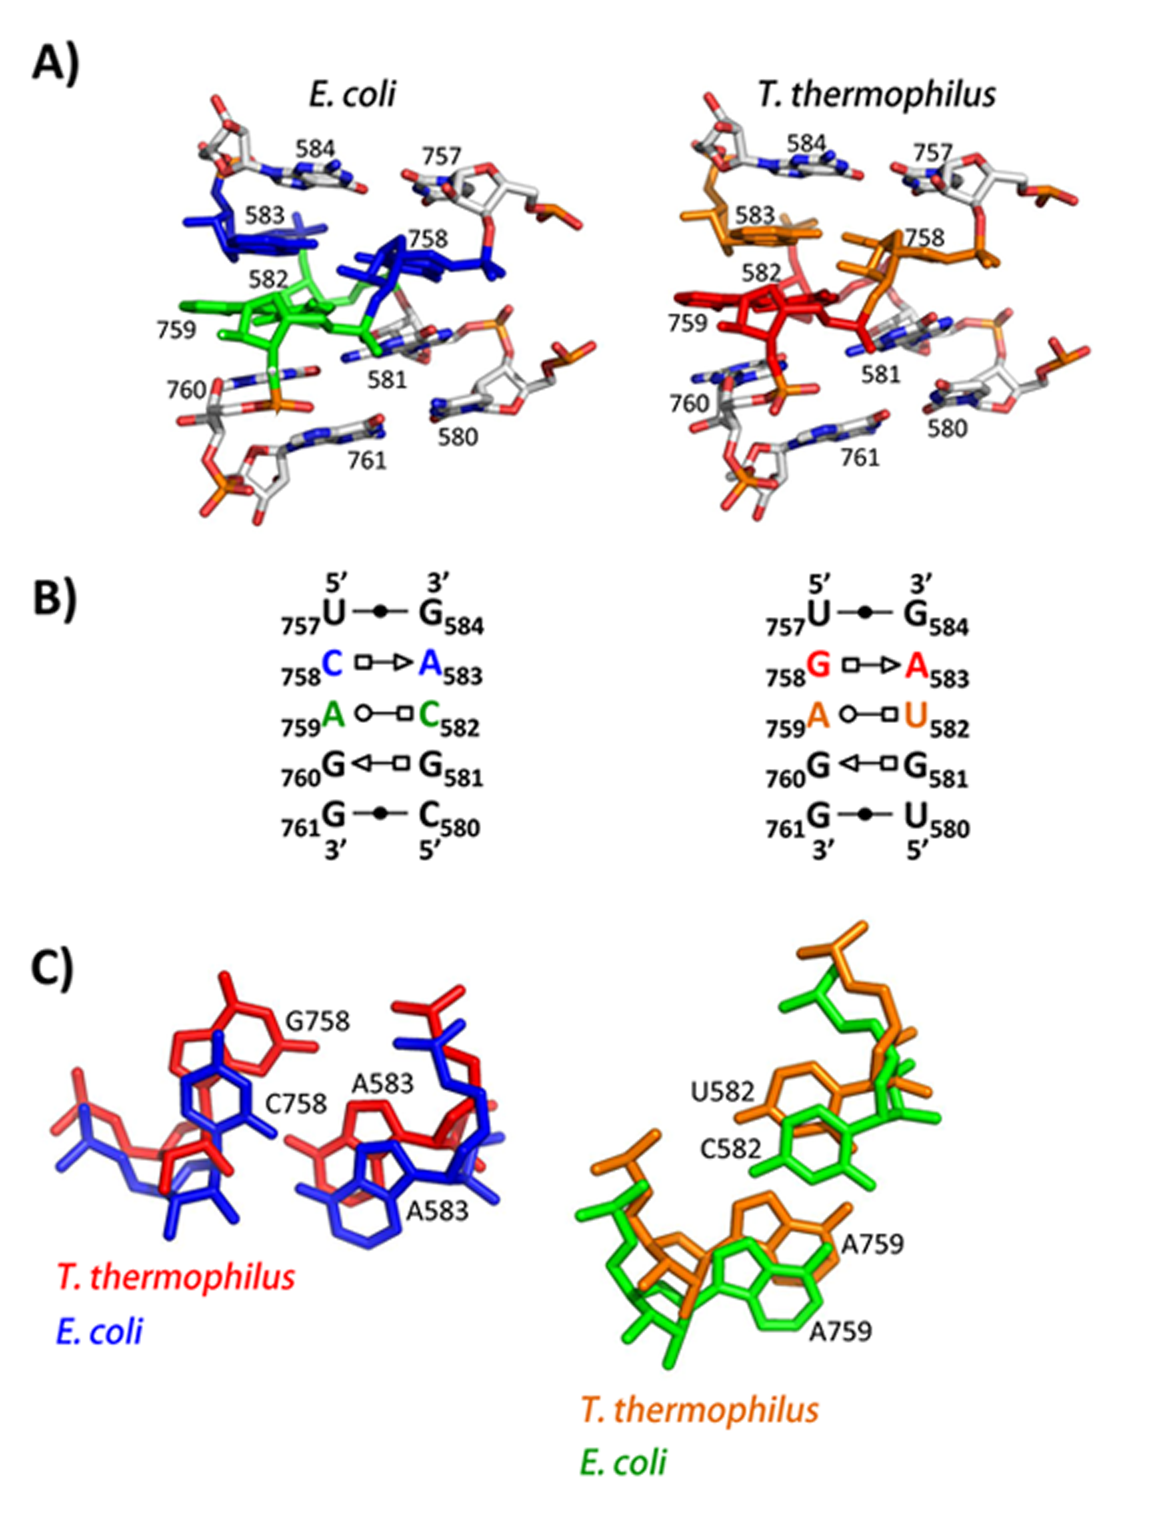
\includegraphics[width=0.5\textwidth]{chapter-1/figs/IL-20}
  \caption{A. 3D structures of IL from helix 20 of 16S rRNA (PDB files 2AW7 [10]
    and 1FJG \cite{Carter2000}. B. 2D annotations showing conserved non-WC basepairs.
    Although they differ in sequence, the two motifs have the same interactions
    and are assigned to the same motif group. C. Superposition of isosteric tWH
    and tSH non-Watson-Crick basepairs from the E. coli and T.thermophilus
  versions of the helix 20 motif.}
  \label{fig:compare-il}
\end{figure}

Grouping structurally similar RNA motif instances in motif families and aligning
corresponding nts among them is crucial to improving bioinformatic methods for
RNA 3D structure prediction based on sequence. In addition to variations in
sequence, recurrent, structurally similar motifs can also differ in the number
of nts they comprise. A key question is which motifs to group together.
Structural analysis based on conserved nt interactions suggests that when the
extra nts found in the larger motifs are bulged out so as not to interact with
the core nts of the motif, and the corresponding core nts form identical
interactions, then the motifs should be assigned to the same group. For example,
some GNRA-type HL have five nts instead of four, but the additional nt is bulged
out without affecting the conformations of the other nts \cite{Nasalean2009b}.
Similarly, there is considerable variation in the number of nts in kink-turn and
C-loop IL motifs, but this variation is largely confined to the looped out nts
on one strand \cite{Lescoute2005}.

\section{Resources for Exploring RNA 3D Structures}

\subsection{RNA 3D Motif Atlas}

These observations provide a framework for classifying recurrent 3D RNA motifs
by geometric similarity. Motifs are assigned to the same motif groups when
corresponding nts form the same interactions, regardless of motif size. This
approach was found to be more successful than relying exclusively on root-mean
square deviations (rmsd) of atomic coordinates and was implemented to construct
the RNA 3D Motif Atlas, a continuously updated resource \cite{Petrov2013}. The
Motif Atlas features automatic extraction of 3D motifs (HL and IL) from the
current non-redundant (NR) dataset of RNA-containing of NDB files and clustering
into structurally similar motifs \cite{Petrov2013}. The Motif Atlas is
comprehensive and representative and can be accessed through NDB or directly at
\url{http://rna.bgsu.edu/rna3dhub/motifs}.

\subsection{Nucleic Acid Database (NDB)}

The NDB (\url{http://ndbserver.rutgers.edu}) is a web portal providing access to
information about 3D nucleic acid structures and their complexes. In addition to
primary data that is archived in PDB, the NDB contains derived geometric data,
classifications of structures and motifs, standards for describing nucleic acid
features, and tools and software for analyzing DNA and RNA. A variety of search
capabilities are available, as are many different types of reports. The NDB was
recently redesigned and continues to evolve to meet the changing needs of RNA
scientists. NDB provides sophisticated search capabilities at the level of whole
structures by a large number of criteria. With the growth of interest in RNA
biology and chemistry, the NDB is offering new RNA-derived data and annotations
and integrating them into the search capabilities
\cite{CoimbatoreNarayanan2014}. For example, NDB is developing finer-grained
search capabilities at the level of individual motifs and interactions. NDB also
provides curated descriptions and links to useful tools and software for RNA
scientists (readers should visit
\url{http://ndbserver.rutgers.edu/ndbmodule/services/softwares.html}).

\subsection{Automated annotation of nt interactions in RNA 3D Structures}

Atomic-resolution 3D structures reveal the architectures of RNA molecules and
the stabilizing local and LR nt interactions. However RNA 3D structures are
complex and difficult for students and non-specialists to comprehend and
interpret. Identifying and classifying individual nt interactions is tedious and
error-prone work when done manually. It is for this reason that computer
programs have been written by several different research groups to automate and
standardize this process \cite{Petrov2011a, Sarver2008a, Yang2003a,
Gendron2001b, Parisien2008a}. The different programs produce annotations that
largely agree with each other; discrepancies occur mainly when annotating
low-resolution structures that are poorly modeled. Annotations of most of the
recurrent nt interactions discussed here are now made available for each new
atomic-resolution experimental RNA 3D structure when it appears in NDB
\cite{Petrov2013}. Annotations are accessible under ``Structural Features'' in
the upper left of each structure summary page of NDB. 

\subsection{Integrating 2D and 3D RNA structural representations}

RNA 2D diagrams illustrate at a glance the folding of the chain to form the
nested Watson-Crick paired helices, identify the domain structure of the RNA and
the sizes and positions of individual HL, IL, and MHJ loops. They can provide
road maps for accessing the 3D structures because it is so easy to find
individual nts in the 2D and to identify neighboring nts in the same helical
elements and loops. What the 2D lacks, of course, are the local and LR non-WC
pairing, stacking and backbone interactions and the spatial relationships
between helical elements. However, interactive computer technology can fill the
gap between the over-simplification of 2D diagrams and the complexity of the 3D. 

The most basic step is the use of color to coordinate the 2D and 3D
representations of RNA molecules, as illustrated for 16S in
Figure~\ref{fig:ec-ssu-2d-3d}. Nts belonging to the same helical element are
colored in 3D as shown in the 2D. Coordinated color-coding of 2D and 3D
structures by helical element facilitates identifying the elements to which
interacting nts belong. In the 3D structure, helical elements distant in the 2D
can be in close proximity and each helical element can interact with several
different elements, not to mention proteins and ligands.  We have provided
SwissPDBViewer and PyMol files with these color codings as supplementary files
to this article to allow readers to visualize \EC{} 16S rRNA on their own
computers. 

The 2D can also be used to rapidly access specific regions of the 3D structure.
In this approach clickable ``hotspots'' are embedded at the locations of
structural features on the online 2D diagram, for example all HL and IL of the
molecule. Clicking on the hotspots brings up an interactive window in which the
3D structure of the selected motif is displayed. Links can be provided to the
motif family to which the motif belongs to access sequence variants of the
motif. One can access 2D diagrams of representative 16S and 23S rRNA molecule
that feature this capability at this link:
\url{http://rna.bgsu.edu/rna3dhub/motifs/2ds}.

While it is possible to represent all local and LR base pairs on a static 2D
representation, the resulting ``circuit diagram'' is difficult to interpret and
comprehend \cite{Lescoute2006a}. An alternative approach is to equip interactive
2D diagrams with sets of controls to selectively display different classes of
interaction by type or location. A prototype of such a display for 16S rRNA can
be accessed here \url{http://rna.bgsu.edu/rna3dhub/pdb/2AW7/2d}.

\subsection{From 1D to 2D to 3D RNA structures}

It will never be possible to solve the 3D structures of all the RNAs we find in
nature at atomic resolution. Fortunately, it may not be necessary to do so as
bioinformatic tools have been developed and are under constant improvement to
predict 2D and 3D RNA structures starting from individual sequences or
alignments of homologous RNA molecules \cite{Leontis2012e}. 

The first step is to predict the 2D structure to identify the helical regions
and define the nts that belong to HL, IL, MJ or linker segments. Dynamic
programming algorithms that make use of a growing database of nearest neighbor
thermodynamic parameters have been refined to make this step quite reliable,
especially when chemical probing or complementary phylogenetic data are
available, i.e. sufficiently diverged homologous sequences \cite{Aigner2012}.
The most commonly used resources are listed in the table provided in
supplemental materials. 

The next step in structure prediction is to identify recurrent HL, IL or MHJ
motifs based on loop sequences identified in the 2D or to carry on de novo
modeling based on energy parameters. Many groups are developing de novo modeling
tools \cite{Rother2012a, Sijenyi2012, Flores2012, Ding2012a, Cao2012}. ``RNA
Puzzles'' has been established to provide CASP-like blind tests of these tools,
leading to rapid progress in RNA 3D modeling \cite{Cruz2012}. Accessible through
NDB is JAR3D, a new on-line tool that is closely linked to the 3D Motif Atlas.
This tool matches user-provided sequences for HL or IL to the most probable
matches of motifs found in the Motif Atlas using observed sequence variations
and considerations of isosteric base pairs to score sequences (see
\url{http://rna.bgsu.edu/main/webapps/jar3d/}).

The next step once the 2D structure is determined and possible 3D structures of
HL and IL are proposed is to predict the conformations of MHJs
\cite{Lamiable2012, Laing2011}.This step is crucial as the MHJ determine the
relative orientations of helical elements in 3D space. It is computationally
challenging. Improvements in the prediction of MHJ in 2D structures also
continue to be made \cite{Liu2011b}.

The final step is to predict tertiary interactions between loops and helical
elements that stabilize the 3D architecture. This step is also very challenging
but is greatly facilitated by sequence analysis when sufficiently diverged and
properly aligned homologs are available for analysis \cite{Michel2000,
Westhof2011}.

\subsection{Conclusion}

We have illustrated, using 16S rRNA, the prevalence of loop nts in structured
RNAs and their central roles in mediating local and long-range interactions that
stabilize the 3D architecture and make possible the specific binding of
proteins, ligands, and other RNA molecules. We have provided a tutorial to
familiarize readers with the most sequence specific of those interactions, the
WC and non-WC base pairs, and showed that by grouping them in geometrically
similar families and isosteric groups, it is possible to interpret and even
predict the sequence variations of recurrent RNA 3D motifs. The distinction
between base combination and base pair geometry was emphasized, because the same
combinations of bases (e.g. UA, AG, CC) can make different types of base pairs.
Base substitutions that preserve the base-pairing geometries maintain functional
structures and are more likely to occur. Annotating interactions is a
prerequisite for grouping 3D motifs into structurally similar groups. This is
how the Motif Atlas is organized. As the number of sequence variants for known
motifs increases, that information can be automatically incorporated to improve
algorithms to predict RNA 3D structure. 

Finally we have provided links to resources to allow readers to deepen their
understanding of RNA 3D structure and access specific information about RNAs of
interest to them. New ways of integrating 2D and 3D representations of
structured RNAs will make it easier for students and scientists to explore and
comprehend the structures, functions, and evolution of these amazing, ancient
molecules. New bioinformatic tools will make it possible to evermore reliably
predict the 2D and 3D structures and possible functions and interactions of new
RNA molecules.
